% !TEX program = xelatex
% basic document config
\documentclass[a4paper,10pt,xetex]{article}
\usepackage[a4paper,top=45mm,right=20mm,bottom=30mm,left=25mm,head=35mm,foot=20mm]{geometry}

% language
\usepackage[german]{babel}

% variable definitions
\providecommand{\documenttitle}{Schlussbericht}
\providecommand{\documentauthors}{Andreas Saurer \\ Benjamin Schneidinger \\ Josef Erben \\ Raffaele Bof \\ Nicolas Loth}
\providecommand{\documentdate}{16.05.2017}
\providecommand{\documentversion}{1.0.0}

% special commands
\newcommand*{\fullref}[1]{\hyperref[{#1}]{\nameref*{#1} (\ref*{#1})}}
\newcommand{\specialcell}[2][c]{%
  \begin{tabular}[#1]{@{}l@{}}#2\end{tabular}}
\usepackage{titlesec}
\usepackage{hyperref}

\titleclass{\subsubsubsection}{straight}[\subsection]

\newcounter{subsubsubsection}[subsubsection]
\renewcommand\thesubsubsubsection{\thesubsubsection.\arabic{subsubsubsection}}
\renewcommand\theparagraph{\thesubsubsubsection.\arabic{paragraph}} % optional; useful if paragraphs are to be numbered

\titleformat{\subsubsubsection}
  {\normalfont\normalsize\bfseries}{\thesubsubsubsection}{1em}{}
\titlespacing*{\subsubsubsection}
{0pt}{3.25ex plus 1ex minus .2ex}{1.5ex plus .2ex}

\makeatletter
\renewcommand\paragraph{\@startsection{paragraph}{5}{\z@}%
  {3.25ex \@plus1ex \@minus.2ex}%
  {-1em}%
  {\normalfont\normalsize\bfseries}}
\renewcommand\subparagraph{\@startsection{subparagraph}{6}{\parindent}%
  {3.25ex \@plus1ex \@minus .2ex}%
  {-1em}%
  {\normalfont\normalsize\bfseries}}
\def\toclevel@subsubsubsection{4}
\def\toclevel@paragraph{5}
\def\toclevel@paragraph{6}
\def\l@subsubsubsection{\@dottedtocline{4}{7em}{4em}}
\def\l@paragraph{\@dottedtocline{5}{10em}{5em}}
\def\l@subparagraph{\@dottedtocline{6}{14em}{6em}}
\makeatother

\setcounter{secnumdepth}{4}
\setcounter{tocdepth}{4}


% font
% \usepackage{titling}
\usepackage[sfdefault]{roboto}
\usepackage[parfill]{parskip}
\usepackage{soul}

% table
\usepackage{array}
\usepackage{multicol}
\usepackage{longtable,tabu,booktabs}

% links
\usepackage{hyperref}
\hypersetup{
            pdftitle={\documenttitle},
            pdfauthor={\documentauthors},
            colorlinks=true,
            linkcolor=[RGB]{74,144,226},
            citecolor=[RGB]{74,144,226},
            urlcolor=[RGB]{74,144,226},
            breaklinks=true}
\urlstyle{same}  % don't use monospace font for urls

% images
\usepackage[font=small,skip=6pt]{caption}
\usepackage{float,graphicx,grffile,wrapfig}
\graphicspath{ {images/} }

\makeatletter
\def\maxwidth{\ifdim\Gin@nat@width>\linewidth\linewidth\else\Gin@nat@width\fi}
\def\maxheight{\ifdim\Gin@nat@height>\textheight\textheight\else\Gin@nat@height\fi}
\makeatother
\setkeys{Gin}{width=\maxwidth,height=\maxheight,keepaspectratio}

\makeatletter
\def\fps@figure{H}
\makeatother

% header and footer
\usepackage{lastpage}
\usepackage{fancyhdr}
\pagestyle{fancy}
\fancyhf{}
\fancyhead[L]{
\includegraphics[height=2cm]{travel-buddy_white}}
\fancyfoot[L]{\fontsize{8}{10}\selectfont\ \documenttitle}
\fancyfoot[R]{\fontsize{8}{10}\selectfont\ Seite\ \thepage\ von\ \pageref*{LastPage}}

\renewcommand{\headrulewidth}{0pt}
\renewcommand{\footrulewidth}{0pt}

% style titles
\usepackage{titlesec}
\titlespacing*{\section}{0pt}{1em}{0pt}
\titlespacing*{\subsection}{0pt}{1em}{0pt}
\titlespacing*{\subsubsection}{0pt}{1em}{0pt}

% configure title page
\title{
  
\includegraphics[width=7cm]{travel-buddy_white}\\[\bigskipamount]
  \documenttitle\\[\bigskipamount]
}

\author{\documentauthors}
\date{\parbox{\linewidth}{\centering%
  IT15TA ZH \hspace*{3cm} Gruppe 3\endgraf\bigskip
  Dokumentversion \documentversion, \documentdate\endgraf
}}


\begin{document}
\shorthandoff{"}

% title page
\maketitle\newpage

% table of contents
{
\hypersetup{linkcolor=black}
\setcounter{tocdepth}{4}
\tableofcontents
}

\newpage

% version log
\section{Versionenlog}\label{versionenlog}

\tabulinesep=1.2mm

\begin{longtabu} to \textwidth { | l | l | X[l] | l | }
  \hline
  \textbf{Datum} & \textbf{Version} & \textbf{Änderung} & \textbf{Author} \\
  \hline
  \endhead

  0.0.6 & 13.05.2017 & Inhalte aus Design übernommen und verbessert & Andi\\
  \hline

  0.0.5 & 13.05.2017 & Inhalte aus Analyse übernommen und verbessert & Andi\\
  \hline

  0.0.4 & 14.05.2017 & Inhalte Resultat hinzugefügt & Raffaele\\
  \hline

  0.0.3 & 13.05.2017 & Inhalte Testbericht Backend hinzugefügt & Beni\\
  \hline

  0.0.2 & 12.05.2017 & Inhalte Testbericht Frontend hinzugefügt & Josef\\
  \hline

  0.0.1 & 12.05.2017 & Inhalte aus Projektskizze übernommen und verbessert & Beni\\
  \hline

  0.0.0 & 12.05.2017 & Dokument erstellt & Andi\\
  \hline
\end{longtabu}
\newpage

% start content
\section{Projektidee}\label{Projektidee}
\subsection{Ausgangslage}\label{Ausgangslage}
Reisen ist ein weltweit verbreiteter Zeitvertrieb und bringt viel Freude und Einblicke in
andere Kulturen mit sich. In vielen Ländern ist es aber auch heute noch schwierig, sich als
Tourist mit einer anderen Muttersprache mit den Einheimischen verständigen zu können. Dies
merkt man auch bei geführten Reisetouren. Häufig sprechen Reiseführer\_innen die Sprache der
Reisegruppe schlecht oder haben einen starken Akzent, so dass man seine Erläuterungen schlecht versteht.

Viele Reisende sind zudem lieber autonom als mit einem Reiseführer auf einer Besichtigungstour
unterwegs. Dadurch fühlt man sich freier und kann selbst entscheiden, wie lange man an einem
Ort verweilen möchte. Mit Uber bietet sich auch eine flexible und kostengünstige Möglichkeit
an, von einem Besichtigungspunkt zum nächsten Punkt zu gelangen.

\subsection{Idee}\label{idee}
Wir entwickeln eine Software, mit welcher Touristen auf einfache Weise verschiedene Besichtigungstouren
durchführen können.
Als Reisende kann man mit der Software für seine Reisedestinationen eine Liste von Touren
zusammenstellen, welche man gerne durchführen möchte. Am jeweiligen Zielort gibt einem die
Software Informationen, wie man von seinem Standort an die Besichtigungspunkte gelangt und
anschliessend folgen Instruktionen, um an die nächsten Punkte zu gelangen. Während der Tour
stellt die App auch Informationen über die Sehenswürdigkeiten bereit.

Für die Wegbeschreibung wird eine Karte eingeblendet, mit welcher sich die Touristin orientieren
und den Weg von Sehenswürdigkeit zu Sehenswürdigkeit ablaufen kann. An jedem Aufenthaltspunkt
der Tour soll die Touristin ein Foto von einem bestimmten Objekt schiessen. Dieses Foto dient
der App zur Verifikation, ob die Touristin sich auch tatsächlich an dem vorgegebenen
Besichtigungspunkt befindet. Wenn der Tourist die Tour vollständig abgelaufen hat und die App
dies durch die gemachten Fotos erkennt, wird ihm eine Zusammenfassung der Tour angezeigt. Diese
kann er nach Bedarf auf seinem Facebook-Profil teilen.

Die Touren werden von anderen Firmen, wie z.B. Reisebüros oder Privatbenutzern, erfasst. Dafür
soll eine Web-Applikation entwickelt werden. Das Erfassen von Touren ist dabei für zertifizierte
Anbieter kostenpflichtig. Den Reisenden wird die Benutzung der App kostenlos zur Verfügung gestellt.

\subsection{Kundennutzen}\label{Kundennutzen}
Die Software bringt folgende Nutzen für Reisende:

\begin{itemize}
\item Die Reisende kann aus einem grossen Angebot von Touren diejenigen auswählen, welche am besten ihre Bedürfnisse decken.
\item Filterkriterien helfen dem Tourist beim Finden von Touren.
\item Der Reisende muss sich keiner Reisegruppe anschliessen und kann mit Hilfe der Software auf einfache Weise eigenständig unterwegs sein.
\item Die Tour wird der Reisenden in ihrer gewünschten Sprache angezeigt.
\item Dank Social-Media-Integration kann der Reisende eine gemachte Tour inkl. seiner Fotos mit seinen Freunden teilen.
\item Die Integration von Uber bietet der Touristin Komfort und Sicherheit. Per Knopfdruck wird innerhalb der TravelBuddy-App
  ein Uber-Taxi angefordert und diesem auch automatisch das Ziel bekanntgegeben. In einem Land mit hoher Kriminalitätsrate ist
  der Transport mit einem Uber-Taxi sicherer als mit einem zufällig auf der Strasse angehaltenen Taxi.
\end{itemize}

Als Kunden für unsere Software zählen aber nicht nur Reisende. Auch die Anwender, welche Touren für die
Software verfassen, sind als Kunden zu betrachten. Dies können Reisebüros, staatliche Tourismusbüros
und viele andere sein. Das Verfassen und Bereitstellen von Touren hat für Unternehmen wie Reisebüros folgende Nutzen:

\begin{itemize}
\item Sie sparen Kosten, da die aufwändige Organisation von Reisetouren im Ausland entfällt.
\item Der Einsatz und die Unterstützung von neuen Reisemöglichkeiten wird junge, technologieversierte Leute anziehen.
\end{itemize}

\subsection{Stand der Technik / Konkurrenzanalyse}\label{StandTechnik}
Es gibt bereits andere Travelguide-Apps, wie z.B. die vom Reiseveranstalter Thomas Cook
Touristik GmbH, welchem auch Neckermann Reisen gehört. Jedoch haben andere Apps nicht den
gleichen Fokus auf digital geführte Reisetouren wie unsere Lösung. Die Thomas-Cook-Travelguide-App
bietet einem das Buchen von geführten Touren an und enthält auch Reiseführerinhalte \cite{TomasCookApp}.

Mit der App ist man jedoch an die Angebote des Reiseveranstalters gebunden. Wir wollen eine
App, bei denen die Anwenderin komplett losgelöst vom Reiseveranstalter eine Tour wählen kann.
Zudem ist Uber nicht in bestehenden Apps integriert, was eine Kernfunktionalität unserer
App ist, mit welcher Besichtigungstouren viel komfortabler werden.

Uber stellt dazu eine Programmier-Schnittstelle zur Verfügung, mit welchem Uber-Fahrten
über fremde Apps abgewickelt werden können (auch ohne, dass die Uber-App selbst auf dem
Gerät installiert ist) \cite{UberApi}. Auch die Social-Media-Integration ist in anderen Apps
nicht gegeben. Wir wollen es den Reisenden auf einfachste Weise ermöglichen, eine gemachte
Tour auf Facebook zu teilen. Dabei werden Informationen über die Tour übermittelt sowie die
persönlichen Fotos gespeichert.

\subsection{Hauptablauf}\label{Hauptablauf}
Der ausführliche Hauptanwendungsfall der Grundidee ist der Tourist, welcher im Urlaub ist und eine Besichtigungstour machen möchte:
\begin{enumerate}
\item Die Touristin startet die TravelBuddy-App, welche sie vorgängig bereits heruntergeladen und installiert hat.
\item Sie sucht nach digital geführten Reisetouren an ihren Standort.
\item Der Tourist wählt die Reisetour aus, welche ihm am besten gefällt und speichert diese.
\item Er betrachtet die Möglichkeiten, um an den Startpunkt der Route zu gelangen.
\item Die App teilt ihm mit, wie er mit öffentlichen Verkehrsmitteln, zu Fuss oder mit Uber-Taxi an das Ziel gelangen kann.
\item Die Touristin wählt die Option Uber-Taxi aus und gibt den genauen Abholort sowie das Datum und die Uhrzeit an, an der sie abgeholt werden möchte.
\item Der Tourist wird zum gewählten Zeitpunkt vom Uber-Taxi abgeholt und an den Startpunkt gefahren. Die Bezahlung des Taxis wird automatisch abgewickelt.
\item Die App erkennt, dass sich die Touristin am Startpunkt der Tour befindet. Die App stellt eine Wegbeschreibung, um ans Zielobjekt zu gelangen sowie detaillierte Informationen über die erste Sehenswürdigkeit bereit.
\item Die App fordert den Kunden auf, eine bestimmtes Objekt an dem Standort zu fotografieren.
\item Sobald die Touristin den Standort fertig besichtigt hat, signalisiert sie dies der App.
\item Die App zeigt nun wieder die Optionen an, wie der Tourist an den nächsten Besichtigungspunkt gelangen kann (Uber-Taxi, öffentliche Verkehrsmittel, Fussmarsch).
\item Der Tourist wählt bspw. "den Weg zu Fuss zurückzulegen".
\item Die App zeigt der Touristin eine Karte an, welche ihn an das nächste Ziel führt.
\item Hat die Touristin den letzten Punkt der Tour besichtigt, wählt sie "Tour beenden" in der App.
\item Die App erstellt eine persönliche Zusammenfassung ihrer Tour, welche auch die von der Touristin gemachten Bilder enthält.
\item Die Touristin wählt, dass sie die zusammengefasste Tour auf ihren Facebook-Account teilen möchte.
\item Die App fügt die Tour-Zusammenfassung auf dem Account des Touristen hinzu.
\item Die App zeigt dem Touristen an, wie er wieder in sein Hotel zurückkommt.
\item Der Tourist wählt wieder die Uber-Taxi-Möglichkeit und wird kurz darauf abholt und in sein Hotel gebracht.
\end{enumerate}

Aus diesem Hauptanwendungsfall leiten sich alle Teilanwendungsfälle ab.

\subsection{Wirtschaftlichkeit}\label{Wirtschaftlichkeit}
Der geschätzte Aufwand beträgt 600 Mannstunden, was etwa 3.5 Mannmonaten entspricht. Die
Entwicklungskosten belaufen sich somit auf 100'000 CHF. Hinzu kommen ca. 16'000 CHF monatlich
für Weiterentwicklungen und Unterhalt. Bei einem Kundenbeitrag von 2'000 CHF pro Monat für
die individuelle Erstellung von Guided Tours mit Travel Buddy beläuft sich der Gewinn bei
10 Kunden auf geschätzte 4'200 CHF monatlich, zuzüglich Werbeeinahmen durch Google Ads.
Somit ergibt ein \textbf{return on investment} nach 24 Monaten.

Durch die flexible Erstellung von Guided Tours lässt sich eine breite Klientel wie beispielsweise
Reiseagenturen, Tourismusbüros und Gewerbeverbände  anziehen, wodurch das Ziel von 10 Kunden
realistisch ist. Ideen für weitere Einnahmequellen wurden evaluiert und können zu einem
späteren Zeitpunkt ausgearbeitet und implementiert werden.


% \section{Analyse}
\subsection{Domänenmodell}
Das folgende Domänenmodell zeigt eine grobe Übersicht der Ausgangslage,
der identifizierten Objekte und Tätigkeiten der Benutzer.

Das Domänenmodell wurde aus dieser Liste von Konzeptklassen abgeleitet:

\begin{longtabu} to \textwidth { | l | X[l] | }
\hline
\textbf{Konzeptklassen} & \textbf{Beispiele} \\\hline
\endhead
Container/Hauptziel         & Trip, Tour                                               \\\hline
Interessante Orte/Wege     & Route, Point of Interest                                \\\hline
Orte                       & City, Country, TouristLocation                           \\\hline
Physische Akteure          & TouristAgency, Tourist                                   \\\hline
Ergebnisse einer Tour      & Photo, TourSummary, TourProgress, SocialMediaPost, Rating \\\hline
Tourüberwachung           & TourProgress, TourTracker                                \\\hline
Vermittlung von Information & Map, Marker                                              \\\hline
\end{longtabu}

\begin{figure}
  \centering
  \includegraphics{domain_model}
  \caption{Domänenmodell}
\end{figure}

\begin{longtabu} to \textwidth { | l | X[l] | }
\hline
\textbf{Objekte} & \textbf{Beschreibung} \\\hline
\endhead

Tourist & Dies ist die Hauptakteurin, der Hauptakteur und Benutzer_in der App. Er wählt eine \textbf{Tour} aus, läuft die \textbf{Route} ab, bringt seine Position durch eine \textbf{Map} in Erfahrung, überprüft seinen Fortschritt (\textbf{TourProgress}) und die Zusammenfassung \textbf{TourSummary}. \\\hline
TouristLocation & Repräsentiert die aktuelle Position der \textbf{Touristin}. \\\hline
TouristAgency & Reisebüros und Tourismusorganisationen erfassen Inhalt (d.h.: \textbf{Touren}, \textbf{Routen} und \textbf{Point of Interests}).\\\hline
Trip & Eine \textbf{Touristin} macht eine Reise (\textbf{Trip}) und hat dort je nach Ort und Stadt mehrere verschiedene \textbf{Touren} zur Auswahl.\\\hline
Tour & Eine \textbf{Tour} ist eine Sammlung von \textbf{Point of Interest}s in einer bestimmten Stadt \textbf{City}, die über eine bestimmte \textbf{Route} miteinander verbunden sind.\\\hline
TourRating & Der \textbf{Tourist} hat die Möglichkeit die \textbf{Tour} am Ende zu Bewertung und einen Kommentar zu hinterlassen. Die \textbf{TouristAgencies} haben Zugang zu diesen Bewertungen.\\\hline
TourProgress & Die \textbf{Touristin} kann aktuelle Metriken während der \textbf{Tour} überprüfen. \\\hline
TourSummary & Am Ende einer \textbf{Tour}, nachdem alle \textbf{Points of Interest} besucht wurden, wird dem \textbf{Touristen} eine Zusammenfassung/Statistik \textbf{TourSummary} über seine absolvierte \textbf{Route}, Anzahl Schritte, Distanz usw\ldots{} angezeigt.\\\hline
Route & Eine \textbf{Route} stellt eine Verbindung von mehreren \textbf{Point of Interests} dar. Eine \textbf{Route} kann mit verschiedenen \textbf{Verkehrsmitteln} absolviert werden.\\\hline
Map & Die Karte zeigt der \textbf{Touristin} mithilfe des \textbf{LocationMarkers} an. \\\hline
LocationMarker & Visuallisiert eine Position auf der Karte \textbf{Map}. \\\hline
City & Enthält mehere \textbf{Trips}. \\\hline
Country & Enthählt mehere Städte (\textbf{City}).\\\hline
Point of Interest & \textbf{Point of Interest} sind geographische Punkte, die eine Sehenswürdigkeit oder sonstige spezielle Eigenschaften bieten. Sie werden von einer \textbf{Route} verbunden. Der \textbf{Tourist} muss beim Absolvieren einer \textbf{Tour} an jedem \textbf{Point of Interest} vorbeikommen und ein \textbf{Foto} schiessen.\\\hline
Means of Transportation & Verschiedene \textbf{Verkehrsmittel} z.B.: Uber, ÖV, Auto, Velo, zu Fuss usw\ldots{}\\\hline
Foto & An jedem \textbf{Point of Interest} schiesst der Tourist mit seiner \textbf{Mobile App} ein \textbf{Foto} des Ortes oder der Sehenswürdigkeit. Wird das \textbf{Foto} akzeptiert, dann gilt der \textbf{Point of Interest} als besucht.\\\hline
SocialMediaPost & Die \textbf{Touristin} hat am Ende einer \textbf{Tour} die Möglichkeit, die Zusammenfassung (\textbf{TourSummary}) inklusive \textbf{Fotos} auf Social-Media-Kanälen zu teilen. \\\hline
\end{longtabu}

\newpage
\subsection{Anwendungsfälle}
\subsubsection{UC 1: Tour auswählen und starten (Priorität 1)}\label{uc-1-user-wuxe4hlt-tour-aus-und-startet-die-tour-priorituxe4t-1}
\subsubsubsection{Primärer Akteur}\label{primuxe4rer-akteur}
Tourist\_in


\subsubsubsection{Stakeholders und Interessen}\label{stakeholders-und-interessen}
\begin{itemize}
  \item Tourist\_in: Will mit einfachen Schritten eine passende Tour finden und starten.
  \item Premium Tour Anbieter\_in: Will seine Tour prominent plaziert haben um öfters ausgewählt zu werden.
\end{itemize}


\subsubsubsection{Vorbedingungen}\label{vorbedingungen}
\begin{itemize}
  \item Tourist\_in ist angemeldet.
  \item Touren sind auf Server erfasst.
\end{itemize}


\subsubsubsection{Erfolgsgarantie}\label{erfolgsgarantie}
Tourist\_in findet eine ansprechende Tour und kann diese starten.


\subsubsubsection{Standardablauf}\label{standardablauf}
\begin{enumerate}
  \item Tourist\_in öffnet app.
  \item Tourist\_in klickt auf neue Tour starten.
  \item System zeigt Auswahl von Touren an.
  \item Tourist\_in öffnet Filter.
  \item Tourist\_in setzt Filter um gewünschte Tour zu finden.
  \item Tourist\_in klickt auf Tour.
  \item System startet Tour.
  \item Tourist\_in begibt sich zum Startpunkt der Tour.
\end{enumerate}


\subsubsubsection{Erweiterungen}\label{erweiterungen}
\begin{enumerate}
  \setcounter{enumi}{3}
  \item
    \begin{enumerate}
      \item Auswahl ist abhängig von gerade populären oder von Premium Anbietern beworbenen Touren.
    \end{enumerate}

  \setcounter{enumi}{6}
  \item
    \begin{enumerate}
      \item App zeigt Detailvorschau an.
      \item Tourist\_in klickt auf Tour starten oder schliessen.
    \end{enumerate}

  \setcounter{enumi}{8}
  \item
    \begin{enumerate}
      \item Die App zeigt der Touristin verschiedene Möglichkeiten an, wie sie zum Startpunkt kommt.
    \end{enumerate}
\end{enumerate}


\subsubsubsection{Spezielle Anforderungen}\label{spezielle-anforderungen}
\begin{itemize}
  \item Filtern der Touren muss flüssig reagieren, Resultate werden sofort angezeigt.
\end{itemize}


\subsubsubsection{Auftrittshäufigkeit}\label{auftrittshuxe4ufigkeit}
Einmal pro Tour.


\subsubsection{UC 2: Route ablaufen und aktuellen Standort auf Karte betrachten (Priorität 2)}\label{uc-2-user-luxe4uft-route-ab-und-sieht-seine-aktuellen-standort-auf-einer-karte-priorituxe4t-2}
\subsubsubsection{Erfolgszenario}\label{erfolgszenario}
Tourist\_in befindet sich im Freien zwischen zwei Punkten auf einer
Route, also einer Teilstrecke der Tour. Die App zeigt dem Benutzer seine
aktuelle Position mit einem Marker (z.B. Punkt) an. Die Touristin verlässt
die Route, der Marker zeigt in Echtzeit die Position an, an der sie sich
befindet. Die App berechnet die neue Route mit der aktuellen Postion als
Ausgangslage. Die Reisende kann also jederzeit die optimale Route
zwischen ihrer aktuellen Position und dem Ziel nachschauen.


\subsubsubsection{Erfolgszenario mit Fallback}\label{erfolgszenario-mit-fallback}
Der Tourist befindet sich auf einer Tour durch eine Altstadt. Die App
zeigt dem Benutzer seine aktuelle Position mit einem Marker (z.B. Punkt)
an, der Marker bewegt sich mit der Touristin mit. Die aktuelle Route zum
nächsten Zwischenziel führt durch ein dicht überdachtes Gebiet. Die App
kann die Position des Benutzers nicht per GPS abfragen, in der Nähe stehen
einige Läden und Restaurants mit WLAN. Die App kann durch eine
Kombination von Standorten von Mobilfunkmasten und WLAN Sendern die
aktuelle Position berechnen. Der Reisende hat kein GPS Signal, aber
sieht sich trotzdem als Punkt auf der Karte in Echtzeit.


\subsubsection{UC 3: Foto machen am Besichtigungspunkt (Priorität 2)}\label{uc-3-user-macht-foto-am-besichtigungspunkt-priorituxe4t-2}
\subsubsubsection{Erfolgszenario}\label{erfolgszenario-1}
An einem Zielpunkt / Besichtigungspunkt angelangt, wird die Touristin aufgefordert, ein Foto von einem vorgegebenen Objekt zu erstellen. Die
App entscheidet danach ob die Informationen des Fotos mit denjenigen im
System gespeicherten übereinstimmen. Stimmt das Resultat, wird der
nächste Besichtigungspunkt angezeigt.


\subsubsubsection{Alternativszenario}\label{alternativszenario}
Befindet sich die Touristin nicht am korrekten Ort, wird sie erneut
aufgefordert das vorgegebene Objekt zu fotografieren.


\subsubsection{UC 4: Bestätigung für Abarbeiten des Punktes erhalten, Route zum nächsten Punkt anschauen (Priorität 2)}\label{uc-4-user-bekommt-bestuxe4tigung-fuxfcr-das-abarbeiten-des-punktes-die-route-zum-nuxe4chsten-punkt-wird-angezeigt.-priorituxe4t-2}
\subsubsubsection{Erfolgszenario}\label{erfolgszenario-2}
Nach dem korrekten validieren der Position des Touristen, zeigt die App
dem Benutzer den nächsten Besichtigungspunkt mit einem Marker auf einer
Karte an. Von seinem aktuellen Standort wird eine vordefinierte Route
zum nächsten Besichtigungspunkt abgebildet. Der Tourist begibt sich zum
abgebildeten Punkt.


\subsubsubsection{Alternativszenario}\label{alternativszenario-1}
Die Touristin möchte die Tour unterbrechen und zu einem späteren
Zeitpunkt fortsetzen. Sie schliesst die App und kehrt nach unbestimmter
Zeit zurück. Die App zeigt dann den letzten Stand und fragt nach der
Weiterführung oder Abbruch der Tour.


\subsubsection{UC 5: Nächste Punkte besichtigen bis Tour zu Ende (Priorität 2)}\label{uc-5-user-besucht-nuxe4chste-punkte-bis-tour-zu-ende.-priorituxe4t-2}
UC1 und UC2 werden solange wiederholt, bis die Touristin am Ende der Tour
ist. Hat sie den letzten Punkt erreicht, wird der Touristin der Abschluss
mit einer Nachricht bestätigt und mit UC 6 fortgefahren.


\subsubsection{UC 6: Statistik der Tour anschauen (Priorität 3)}\label{uc-6-user-sieht-statistik-der-tour.-priorituxe4t-3}
Nach erfolgreichem erreichen des Zielpunktes und dem Abschluss der Tour,
wird dem Tourist eine Übersicht mit Statistiken, wie z.B. der total
zurück gelegten Distanz und totale Schritte, angezeigt. Durch einen klick
kann der Tourist Fotos, die Statistik und eine Mitteilung auf den
sozialen Medien teilen.


\subsection{Anwendungsfalldiagramm}\label{anwendungsfalldiagramm}
Das folgende Anwendungsfalldiagramm zeigt eine Übersicht von allen Anwendungsfällen in Relation mit den Aktoren, welche identifiziert wurden.

\begin{figure}
  \centering
  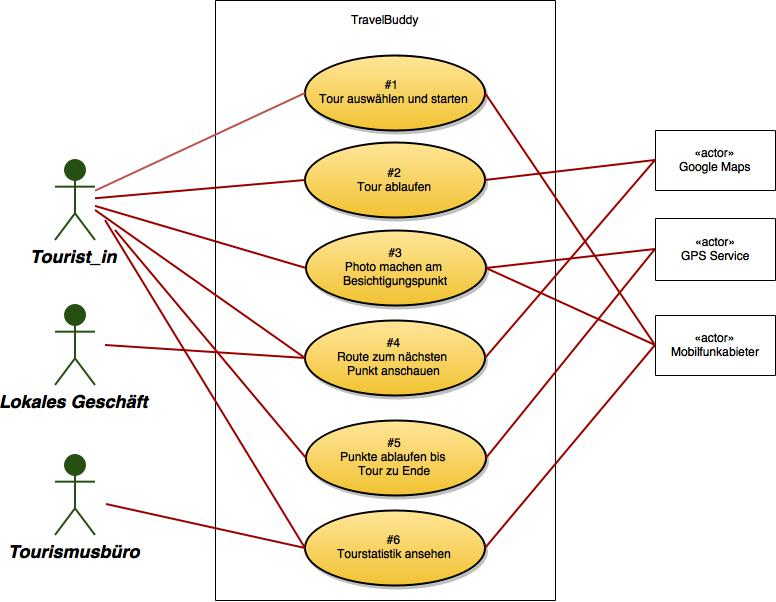
\includegraphics{Anwendungsfalldiagramm}
  \caption{Anwendungsfalldiagramm}
\end{figure}


\section{Design}
\section{Design}\label{design}
\subsection{Backend Design}\label{backend-design}
\subsubsection{Service API}\label{service-api}
Die API ist als Webservice aufgebaut welcher funktionale Requests beantworten kann. Es wird kein direkter Datenzugriff
\"uber CRUD Methoden zur Verf\"ugung gestellt. Die Business-Logik wird wenn m\"oglich vollst\"andig im Service
abgehandelt. So ist die Funktionalit\"at des ganzen Systems gekapselt und unabh\"angig von allenfalls in der Zukunft
weiteren entwickelten Clients.

Nachfolgend sind alle geplanten Service Methoden nach Controller gruppiert aufgelistet. Eine
interaktive Version ist unter \fullref{swagger} verlinkt.

\begin{figure}
  \centering
  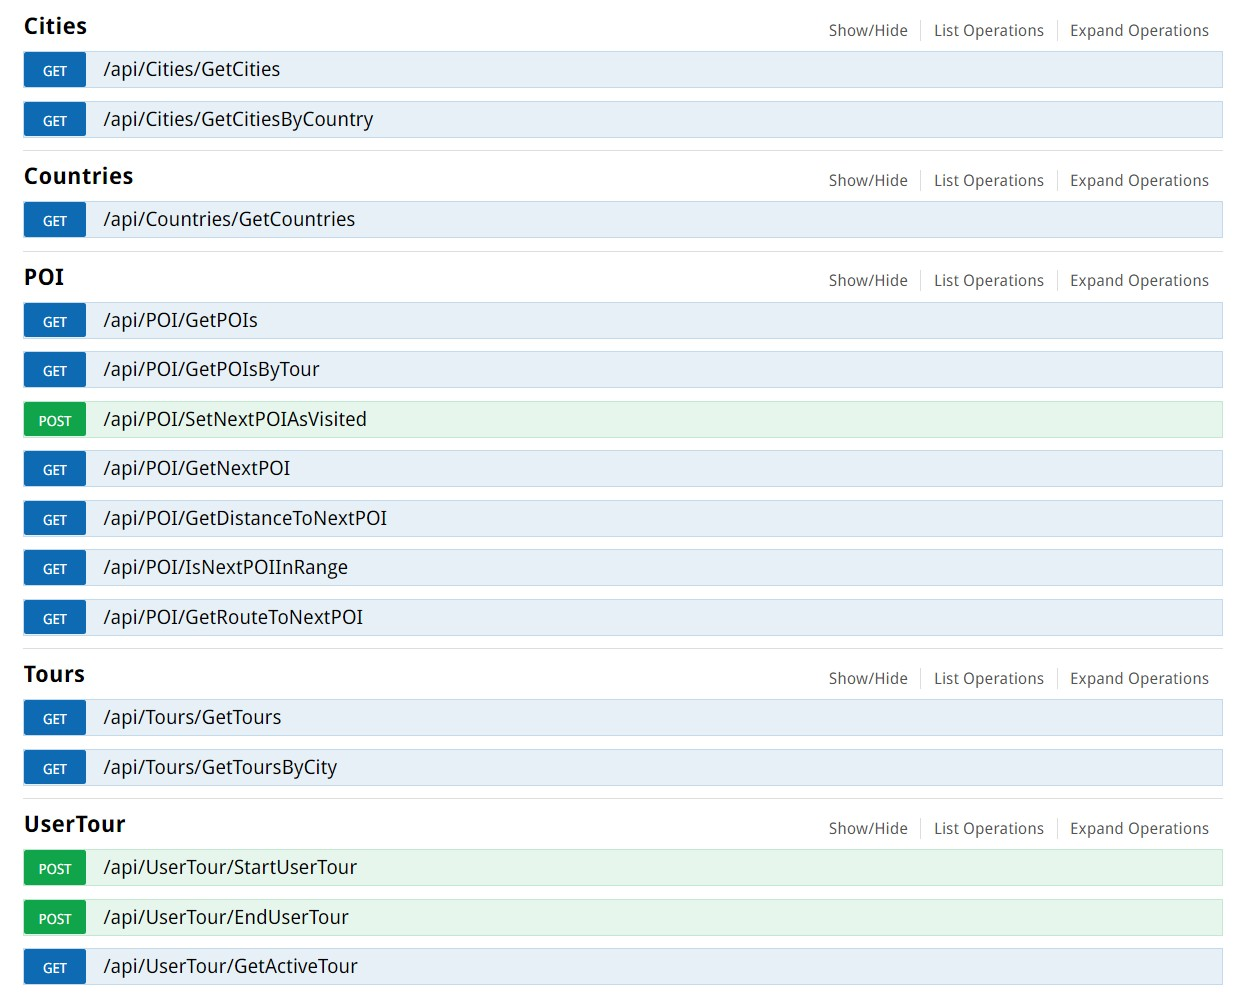
\includegraphics{swagger_schlussbericht}
  \caption{Übersicht API}
\end{figure}

\newpage
Controller:

\begin{longtabu} to \textwidth { | l | X[l] | }
\hline
\textbf{Controller} & \textbf{Beschreibung} \\
\hline
\endhead

Cities & Implementiert alle Funktionalit\"aten zum Abfragen und \"Andern von
  St\"adte-Daten\\ \hline
Countries & Implementiert alle Funktionalit\"aten zum Abfragen und \"Andern von
  L\"ander-Daten\\ \hline
POI & Implementiert alle Funktionalit\"aten zum Abfragen und \"Andern von Point of
Interests, welche durch eine Tour verkn\"upft sind. Zudem alle Funktionalit\"aten zum Abfragen und \"Andern von UserPOIs.
  Ein User POI ist ein Point of Interest welcher von einem Benutzer besucht wurde oder
  welcher ein Benutzer im Rahmen seiner gestarteten Tour als n\"achstes besuchen muss.\\\hline
Tours & Implementiert alle Funktionalit\"aten zum Abfragen und \"Andern von Touren. Zudem alle Funktionalit\"aten zum Abfragen und \"Andern von UserTouren.
  Eine UserTour ist eine Tour die von einem Benutzer gestartet wurde.\\\hline
\end{longtabu}

Die API wurde gegenüber dem Design-Entwurf vereinfacht, vereinheitlicht und die Unterscheidungslogik zwischen z.B. POI und UserPOI wurde nach aussen weggekapselt.
Nicht mehr vorhandene Methoden in der aktuellen Version sind mit removed gekennzeichnet.

Methoden:

\begin{longtabu} to \textwidth { | l | X[l] | }
\hline
\textbf{Methode} & \textbf{Beschreibung} \\
\hline
\endhead

api/Cities/GetCities &
Liefert eine Liste aller vorhandenen St\"adte.\\\hline
api/Cities/GetCitiesByCountry &
Liefert eine Liste aller vorhandenen St\"adte in einem bestimmten Land.\\\hline
  api/Countries/GetCountries &
Liefert eine Liste aller vorhandenen L\"ander.\\\hline
api/POI/GetPOIs &
Liefert eine Liste aller vorhandenen POIs.\\\hline
api/POI/GetPOIsByTour &
Liefert eine Liste aller POIs zu einer bestimmten Tour.\\\hline
api/POI/SetNextPOIAsVisited &
Markiert den n\"achsten POI, den ein bestimmter Benutzer aufgrund seiner aktiv gestarteten
  Tour besuchen muss, als besucht.\\\hline
  api/POI/GetNextPOI &
Liefert f\"ur eine Benutzer-ID den n\"achsten POI zur\"uck, den der Benutzer besuchen
  muss.\\\hline
  api/POI/GetDistanceToNextPOI &
Gibt aufgrund von Geokoordinaten und einer Benutzer-ID die Distanz bis zu einem n\"achsten POI
  den der Benutzer mit seiner gestarteten Tour besuchen muss.\\\hline
api/POI/IsNextPOIInRange &
Gibt aufgrund von Geokoordinaten und einer Benutzer-ID zur\"uck, ob die Koordinaten gen\"ugend
  nahe am n\"achsten POI, den der Benutzer mit seiner gestarteten Tour besuchen muss, ist.

Die erlaubte Distanz kann als optionaler Parameter mitgegeben werden.\\\hline
  api/POI/GetRouteToNextPOI &
Liefert aufgrund einer Benutzer-ID die Route als einzelne Navigationspunkte zum n\"achsten
  POI, den der Benutzer mit seiner gestarteten Tour besuchen muss.\\\hline
api/POI/GetDistanceToPOI (removed) &
Gibt aufgrund von Geokoordinaten die Distanz bis zu einem bestimmten POI zur\"uck.\\\hline
api/POI/IsPOIInRange (removed)&
Gibt aufgrund von Geokoordinaten zur\"uck, ob diese gen\"ugend nahe an einem POI sind. Die
  erlaubte Distanz kann als optionaler Parameter mitgegeben werden. \\\hline
api/UserPOI/CheckUserTourPOI (removed) &
Markiert einen bestimmten POI in einer UserTour als besucht.\\\hline
api/UserPOI/CheckPOI (removed) &
  Markiert einen bestimmten POI f\"ur eine angegebene Tour und eine definierte Benutzer-ID als
  besucht.\\\hline
api/Tours/GetTours &
Gibt alle vorhandenen Touren zur\"uck.\\\hline
api/Tours/GetToursByCity &
Gibt alle vorhanden Touren in einer bestimmten Stadt zur\"uck.\\\hline
api/UserTour/StartUserTour &
Startet eine definierte Tour f\"ur einen bestimmten Benutzer. Liefert direkt eine Auflistung
  aller POIs und Routenpunkte dieser Tour zur\"uck.\\\hline
api/UserTour/EndUserTour &
Beendet die aktive UserTour f\"ur einen bestimmten Benutzer. \\\hline
api/UserTour/GetActiveTour &
Gibt die aktive Tour des Benutzers zur\"uck.\\\hline
\end{longtabu}

\subsubsubsection{Versionierung der API}\label{versionierung-api}
F\"ur gr\"ossere \"Anderungen an der API soll aus Kompatibilit\"atsgr\"unden eine neue Version erstellt und parallel zu
\"alteren Versionen deployt werden. Swashbuckle bietet auch hierf\"ur die notwendige Funktionalit\"at zur Versionierung
an.

\subsubsection{Externe Frameworks}\label{externe-frameworks}
Zur Implementierung von architektonischen und business-funktionalen Anforderungen, die nicht bereits mit ASP.NET MVC und
Web API abgedeckt sind, sollen bereits bestehende Libraries und Frameworks verwendet werden. Die nachfolgende Tabelle
listet die zu verwenden Frameworks auf:

\begin{longtabu} to \textwidth { | l | l | l | X[l] | }
\hline
\textbf{Framework} & \textbf{Version}  & \textbf{Typ} & \textbf{Beschreibung} \\
\hline
\endhead

Google Maps API &
0.65 &
Funktional &
Wird verwendet um die funktionalen Anforderungen wie Routenberechnung usw. zu
  implementieren.\\\hline
Ninject &
3.2.0 &
Architektur &
Ninject ist ein Dependency Injection Framework, welches eine Integration f\"ur ASP.NET
  anbietet. Mit Dependency Injection sollen die einzelnen Repositories den Controllern zur Verf\"ugung gestellt werden.
  Dadurch soll ebenfalls gew\"ahrleistet werden, dass pro Request und Repository nur genau eine Datenbankverbindung
  aufgebaut und dann auch wieder sauber geschlossen wird. So werden Performance- und Datenkonsistenzprobleme, sowie
  Probleme mit nicht geschlossenen Datenbankverbindungen vermieden.\\\hline
Swashbuckle &
5.2.1 &
Architektur &
Swashbuckle erm\"oglicht das automatische Generieren und Anzeigen von Swagger Interface
  Descriptions zur Laufzeit. Mit Hilfe dieser Descriptions k\"onnen die Services einfacher integriert werden, indem zum
  Beispiel die Datenobjekte oder Proxy-Klassen auf Konsumentenseite automatisch generiert werden k\"onnen.\\\hline
Log4Net &
2.0.8 &
Nicht-Funktional &
Framework zum Loggen von Fehlern, Warnungen und Debug-Informationen an verschiedene
  Appenders wie Datenbank oder Logfile.\\\hline
\end{longtabu}


\subsubsection{Architektur}\label{backendarchitektur}
Das nachfolgende Diagramm zeigt die Detail-Architektur des Backends. Weitere grundlegende
Informationen zum eingesetzten Technologie-Stack befinden sich im Dokument Anforderungsanalyse.

\begin{figure}
  \centering
  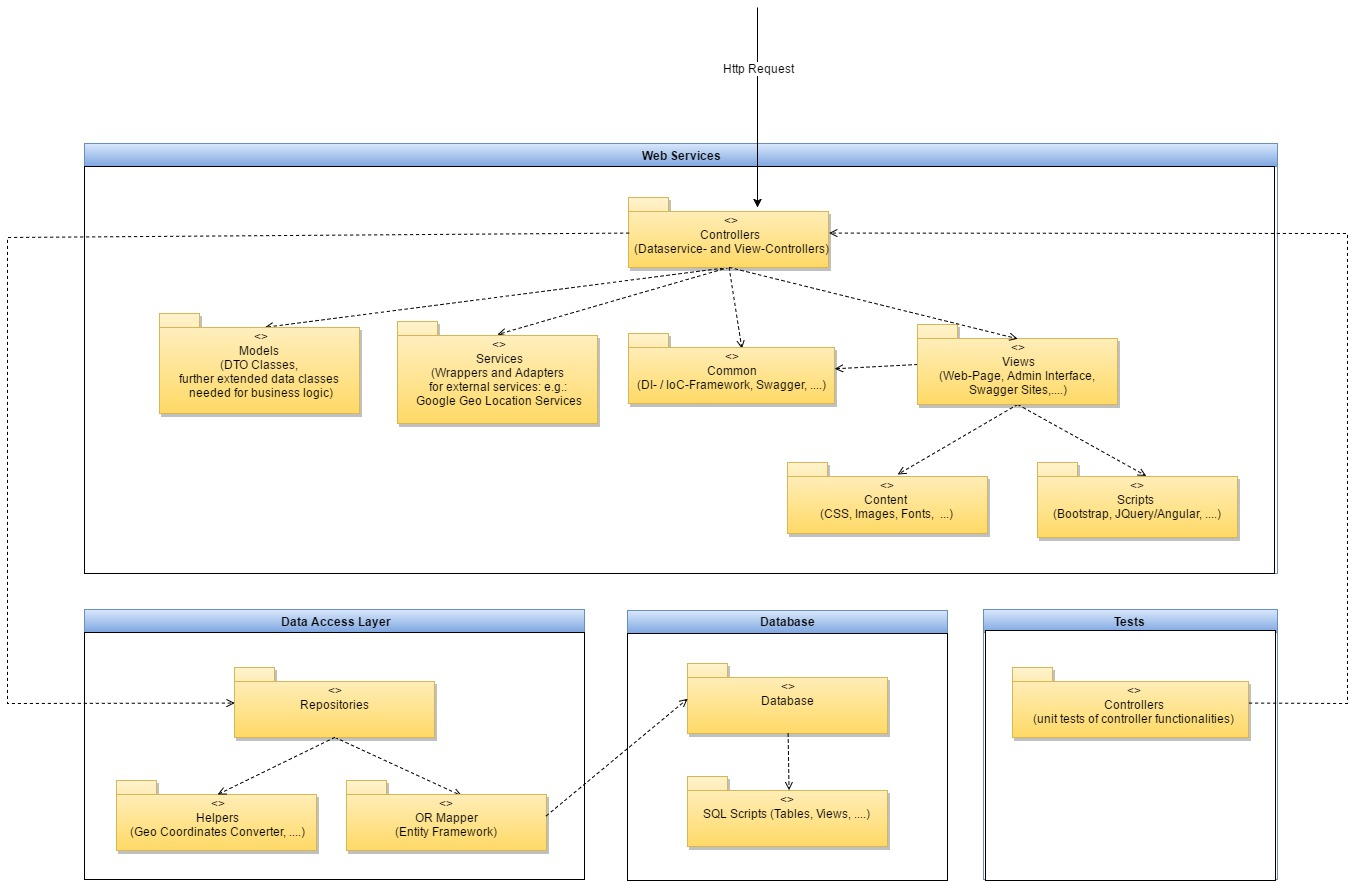
\includegraphics{backend_architektur_schlussbericht}
  \caption{Backend Architektur}
\end{figure}

\newpage
\begin{longtabu} to \textwidth { | l | l | X[l] | }
\hline
\textbf{Layer} & \textbf{Package}  & \textbf{Beschreibung} \\
\hline
\endhead

Web Services &
Controllers &
Controllers beinhaltet alle WebAPI- sowie MVC-Controller, welche die ankommenden Requests
  bearbeiten.

Ein Controller hat mindestens eine Methode und wird \"uber eine spezifische Sub-Url
  aufgerufen. ASP.NET WebAPI/MVC \"ubernimmt das automatische Mapping des ankommenden Requests mit den entsprechenden
  Parametern inkl. Request-Type \ und findet die passende Methode des Controllers, die diesen Request verarbeiten kann.
  Ein API Controller liefert nur Daten in JSON oder XML Format und keine darstellungsspezifischen Informationen.

Zu einem sp\"ateren Zeitpunkt k\"onnen f\"ur die Implementierung der Web-Applikation als
  Administrations-Interface MVC-Controller erstellt werden welche eine entsprechende HTML View zur\"uckgeben. S\"amtliche
  Daten sollen aber auch hier dynamisch \"uber API-Controller mit AJAX-Requests geladen werden. Es sollen keine Seiten
  mit Daten serverseitig gerendert werden.\\\hline
Web Services &
Models &
Dieses Paket beinhaltet alle Model-Klassen welche in den Webservices ben\"otigt werden. Diese
  Klassen unterscheiden sich durch Attribut-Erg\"anzungen (z.B. f\"ur aggregierte oder aufgeschl\"usselte Datenfelder)
  gegen\"uber den vom Entity-Framework generierten Datenklassen welche prim\"ar die Datenbankstruktur abbilden.

Hier befindet sich auch die Funktionalit\"at zum Mappen der Entity-Framework-Datenklassen auf
  DTO Klassen.\\\hline
Web Services &
Services &
Hier sind alle Adapter- und Wrapperklassen f\"ur externe Service angesiedelt, welche f\"ur
  weitere Funktionalit\"aten vom Backend aufgerufen werden.\\\hline
Web Services &
Common &
Dies beinhaltet alle Klassen und Funktionalit\"aten welche \"uber das ganze Projekt hinweg
  ben\"otigt werden. Hierbei handelt es sich zum Beispiel um die ganze Dependency Injection oder Swagger
  Funktionalit\"at.\\\hline
Web Services &
Views &
Zu einem sp\"ateren Zeitpunkt soll neben den Datenservices auch eine Webapplikation erstellt
  werden, welche das Administrieren der Daten erm\"oglichen soll. Hierf\"ur k\"onnen in diesem Package HTML Views
  erstellt werden.\\\hline
Web Services &
Content &
Content beinhaltet den Content der f\"ur die Darstellung der Views ben\"otigt wird wie zum
  Beispiel CSS-Files, Bilder, Fonts usw.\\\hline
Web Services &
Scripts &
Hier werden alle Skripts abgelegt die client-seitig ben\"otigt werden. Es handelt sich hierbei
  vor allem um selbst erstellte Javascript-Funktionalit\"aten und Javascript Frameworks wie JQuery, Angular, Bootstrap
  usw. Die Details zur Implementierung des Webinterfaces werden zu einem sp\"ateren Zeitpunkt genauer definiert.\\\hline
Data Access Layer &
Repositories &
Grunds\"atzlich existiert f\"ur jede Datenklasse aus der Datenbank ein Repository, welche die
  Daten (teil-)aggregiert und funktional zur Verf\"ugung stellt. Dadurch ist die Wiederverwendbarkeit grundlegender oder
  kombinierter Datenabfragen gew\"ahrleistet.\\\hline
Data Access Layer &
Helpers &
Zum Beispiel f\"ur das Umwandeln der Koordinaten-Angaben vom MSSQL-Format in einzelne
  Werteangaben f\"ur L\"angen- und Breitengrade werden Helferklassen ben\"otigt, welche hier angesiedelt sind.\\\hline
Data Access Layer &
OR Mapper &
Als klassischer OR Mapper wird das Entity Framework mit dem Database First Vorgehen verwendet.
  Dies bedeutet, dass basierend auf der Datenbank automatisch Proxy-Datenklassen vom Entity-Framework generiert
  werden.\\\hline
Database &
Database &
Das Datenbankprojekt wird vollst\"andig als MSSQL Datenbank Projekt umgesetzt. Damit werden
  automatisch \"Anderungen an den SQL Dateien im Projekt getrackt und es k\"onnen unter Beachtung dieser \"Anderungen
  automatisch Datenbank Installations-Packages (DACPAC) generiert werden, welche den initialen Stand oder ein Delta
  beinhalten.\\\hline
Database &
SQL Scripts &
Die eigentlichen SQL Skripts f\"ur Tables, Views oder weitere Datenbank-Elemente.\\\hline
Tests &
Controllers &
Dieses Testprojekt implementiert alle Unit-Tests zum automatischen Testen der WebAPI
  Controller-Funktionalit\"aten. \\\hline
\end{longtabu}

\subsubsubsection{Ablauf eines Request und Datenfluss aus technischer Sicht}\label{ablauf-request}
Der nachfolgende Prozess zeigt den programmatischen Standardablauf eines Request im Backend, inklusive dem Datenfluss
von der Datenbank bis zum Inhalt in der HTTP-Response, auf:

\begin{enumerate}
  \item
    Der Controller erh\"alt einen Request. Bei der Instanzierung des Controller werden automatisch \"uber Dependency Injection
    die ben\"otigten Repositories instanziert und mitgegeben. Ein Repository erstellt bei der Instanzierung automatisch
    eine Datenbankverbindung. F\"ur einen Request wird so pro Repository nur eine einzige Datenbankverbindung aufgebaut, da
    auch nur eine Repository-Instanz erstellt wird.
  \item
    Die Repository-Klasse extrahiert die ben\"otigten Daten mit LINQ-Queries und gibt diese immer als IQueryable
    R\"uckgabewert zur\"uck. Damit lassen sich einzelne Repository-Abfragen theoretisch auch hintereinanderschalten oder es
    sind weitere Operationen auf dem Datensatz m\"oglich.
  \item
    Die Daten werden \"uber das Datenmodel vom Entity-Framework beim Materialisieren des LINQ-Queries geladen.
  \item
    Die Controller-Funktion erstellt eine Instanz des DTO. Dies geschieht entweder mit automatischen Mapping \"uber
    Reflection f\"ur gleiche Felder wie die Datenklassen des Entity Framework Modells oder falls ben\"otigt mit manuellen
    Mapping \"uber eine wiederverwendbare Lambda Function Expression f\"ur einzelne oder mehrere Properties. Diese kann
    direkt auf das erhaltene IQueryable als Select-Befehl angewendet werden.
  \item
    Der Controller gibt das Resultat zusammen mit einem Statuscode zur\"uck.
  \item
    Die Repository Instanz wird nicht mehr ben\"otigt. Die Datenbankverbindung wird geschlossen und die Instanz disposed.
\end{enumerate}

\newpage
\subsubsubsection{Dependency Injection}\label{dependency-injection}
Als Dependency Injection Framework f\"ur die Umsetzung des Inversion of Control Patterns wird Ninject eingesetzt.
Ninject bietet eine statische Konfiguration zum Binden von Interfaces an bestimmte Klassen welche bei einer solchen
Anfrage instanziert werden m\"ussen. Eine solche Implementierung bietet eine bessere Performance als wenn die zu
instanziierenden Klassen im ganzen Projekt zuerst gesucht werden m\"ussen. Die Services welche injected werden, sollen
als One-Per-Request Modul definiert sein.


Da ein Controller von der erfolgreichen Instanzierung seines ben\"otigten Repositories abh\"angig ist (strong-coupled),
w\"are in einer n\"achsten Version eine Implementierung der Repositories als Lazy-Object sinnvoll. Dadurch w\"urde die
Instanzierung erst beim ersten Zugriff innerhalb des Controllers geschehen und es k\"onnte bei einem Problem spezifisch
darauf reagiert werden. Bei der direkten Injection ist dies nur begrenzt m\"oglich, da dann entweder vorher einen Fehler
geworfen wird oder aber die injezierten Parameter als Null daherkommen.

\subsubsubsection{Logging}\label{logging}
Das Logging wird mit Hilfe der Log4Net Library implementiert. Geloggt werden soll in t\"agliche Rolling-Logfiles, was
als Appender in Log4Net konfiguriert werden kann.

\subsubsubsection{Security}\label{security}
Das Thema Security inklusive Authentifizierung und Authentisierung von Benutzern, die Implementierung von verschiedenen
Rollen, das Verschl\"usseln der Kommunikation usw. soll f\"ur die erste Version des Backends nicht beachtet werden.

\subsubsubsection{Testing}\label{testing}
F\"ur die Implementierung von Unit-Tests der Controller, muss ein Controller manuell instanziert werden k\"onnen. Dies
bedeutet, dass jede Controller-Klasse einen leeren Konstruktor implementieren muss, in welchem die ben\"otigten
Repositories manuell instanziert werden.

\subsubsubsection{Swagger}\label{swagger}
\"Uber Swashbuckle wird die automatische Generierung von Swagger Interface Definitions implementiert.

\begin{longtabu} to \textwidth { | X[l] | X[l] | }
\hline
\textbf{Url} & \textbf{Content} \\\hline
\endhead

\url{http://travelbuddy5.azurewebsites.net/swagger/ui/index} & Url zum Aufruf der
  generierten Seite inklusive Methoden zum direkten, parametrisierten Aufruf.\\\hline
\url{http://travelbuddy5.azurewebsites.net/swagger/docs/v1} & Url zum Aufruf der generierten
  JSON Interface Definition. Die Versionsnummer kann je nach Version der API angegeben werden.\\\hline
\end{longtabu}

\newpage
\subsubsection{Klassendiagramme und Klassenverantwortlichkeiten}\label{klassendiagramme}
Dieses Diagramm zeigt das Zusammenspiel der Controller mit den jeweiligen Repositories.

\begin{figure}
  \centering
  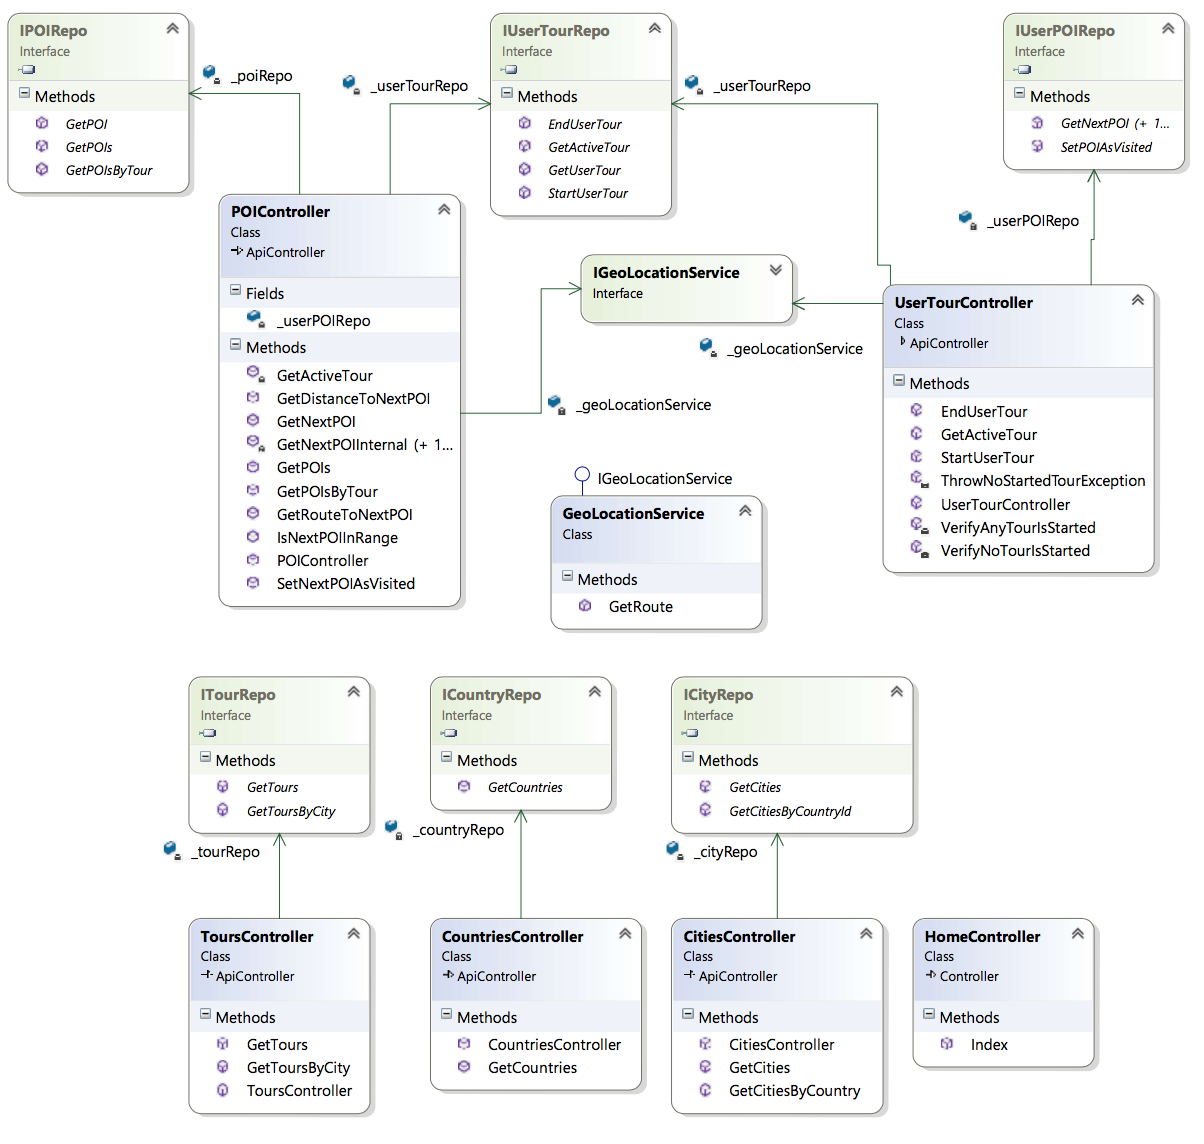
\includegraphics{klassendiagramm_backend_schlussbericht1}
  \caption{Klassendiagramm mit Zusammenspiel der Controller und den jeweiligen Repositories}
\end{figure}

Die Controller weisen die in der Service API beschriebenen Funktionalit\"aten und Verantwortlichkeiten auf. Sie
behandeln alle ankommenden Requests und verwenden daf\"ur 1-n Repositories (da es sich nicht um reine CRUD Controller
handelt, k\"onnen auch mehrere Repositories verwendet werden) um die Daten aus der Datenbank zu holen und beliebige
Services, wie zum Beispiel den GeoLocationService, welcher einen Wrapper f\"ur die Google Maps Geo Location Services
implementiert. Services und Repositories werden wie bereits beschrieben \"uber Dependency Injection den Controllern zur
Verf\"ugung gestellt. Der HomeController dient als Einstiegspunkt der WebApplikation und ist daher kein API Controller.
Er liefert eine HTML View zur\"uck.

Die DTO Klassen sind erweiterte Datenklassen basierend (aber nicht vererbt) auf den vom Entity-Framework automatisch
generierten Datenklassen. Dies erm\"oglicht eine Erg\"anzung der Attribute um aggregierte oder separierte Werte.

\begin{figure}
  \centering
  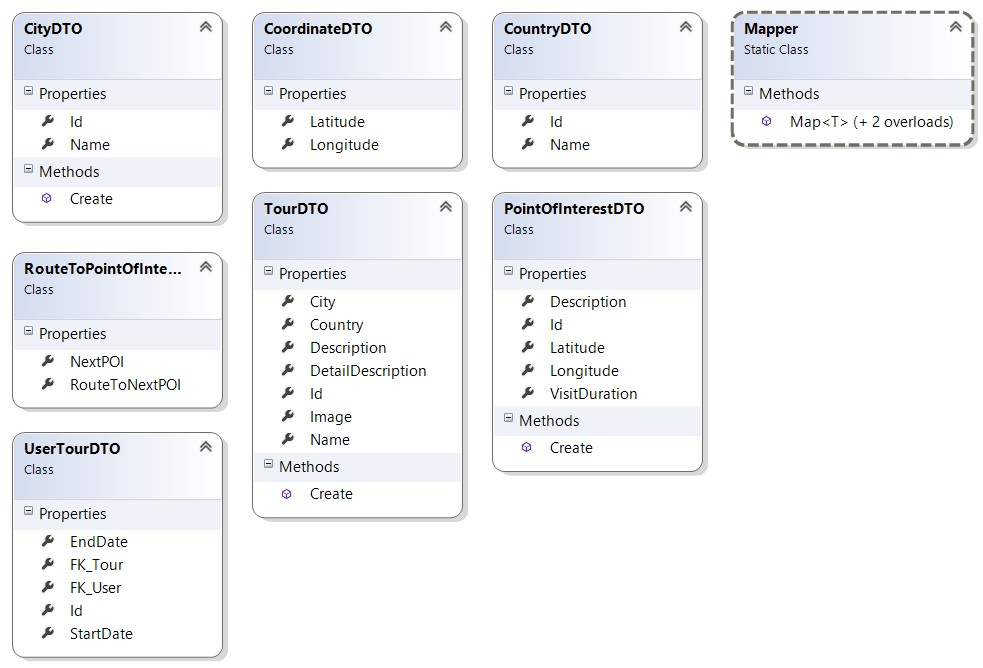
\includegraphics{klassendiagramm_backend_schlussbericht2}
  \caption{Klassendiagramm DTO Klassen}
\end{figure}

Hier speziell zu erw\"ahnen sind die statische Mapper Klasse und der wiederverwendbare POIMapper. Die generische Mapper
Klasse mappt mit Hilfe von Reflection eine Datenklasse des Entity-Frameworks direkt auf gleichnamige Felder der
gew\"unschten DTO Klasse. Diese Funktionalit\"at kann f\"ur alle Felder verwendet werden die eins zu eins in beiden
Datenklassen vorhanden sind und den gleichen Datentypen besitzen. Ein manuelles Mappen dieser Felder ist damit nicht
mehr notwendig. Die DTO Klassen stellen die manuelle Mapping-Logik z.B. f\"ur das Aufsplitten der Geo-Koordinaten in
Latitude und Longitude in wiederverwendbarer Form bereit. Sie liefern eine LINQ Function-Expression zur\"uck, welche die
Mapping-Logik definiert.

\newpage
Die Repository Klassen implementieren das jeweilige von den Controllern von aussen her verwendete Interface.

\begin{figure}
  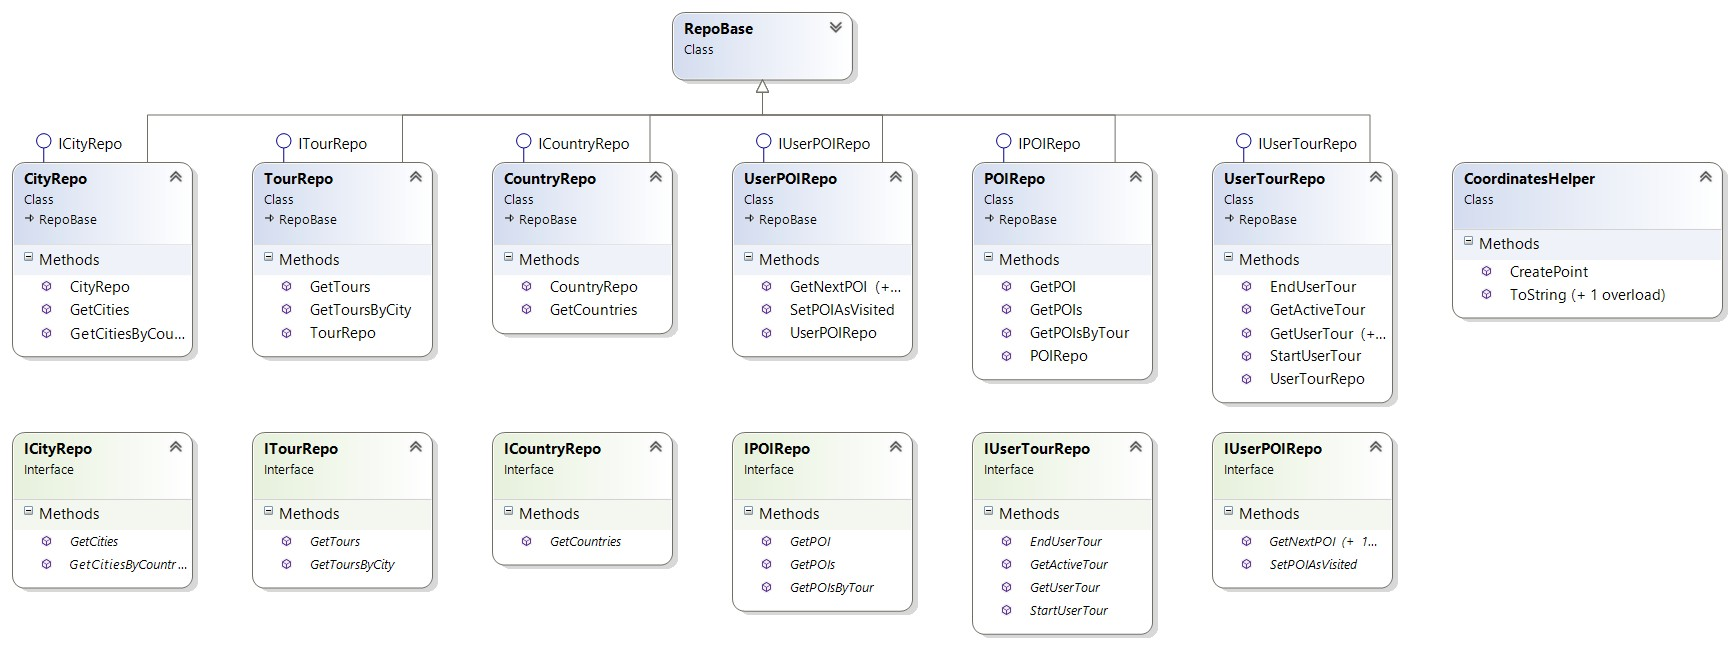
\includegraphics{klassendiagramm_backend_schlussbericht3}
  \caption{Klassendiagramm der Repository Klassen}
\end{figure}

Die einzelnen Repositories implementieren den Zugriff \"uber LINQ-Queries auf die vom Vorbild der Datenbank generierten
Datenklassen\--Objekte. Sie sind alle von der Klasse RepoBase abgeleitet. RepoBase \"offnet bei der Instanzierung
automatisch eine Datenbankverbindung und stellt diese Verbindung den abgeleiteten Klassen zur Verf\"ugung. Die fachlichen und
funktionalen Verantwortlichkeiten werden analog zu den Zust\"andigkeiten der Controller implementiert. Im Kapitel
Service API werden daf\"ur die notwendigen Begriffe und Unterteilungen detailliert erl\"autert.

Speziell ist hier die Klasse CoordinatesHelper.
Der CoordinatesHelper \"ubersetzt das MSSQL Datenbankformat der Geo-Koordinaten in einzelne ben\"otigte Werte wie
L\"angen- und Breitengrad und umgekehrt.

\newpage
\subsubsection{Entity Relationship Diagram}\label{erm}
Als Erg\"anzung und zum besseren Verst\"andnis der Zusammenh\"ange nachfolgend das Diagramm des Datenbankmodels.

\begin{figure}
  \centering
  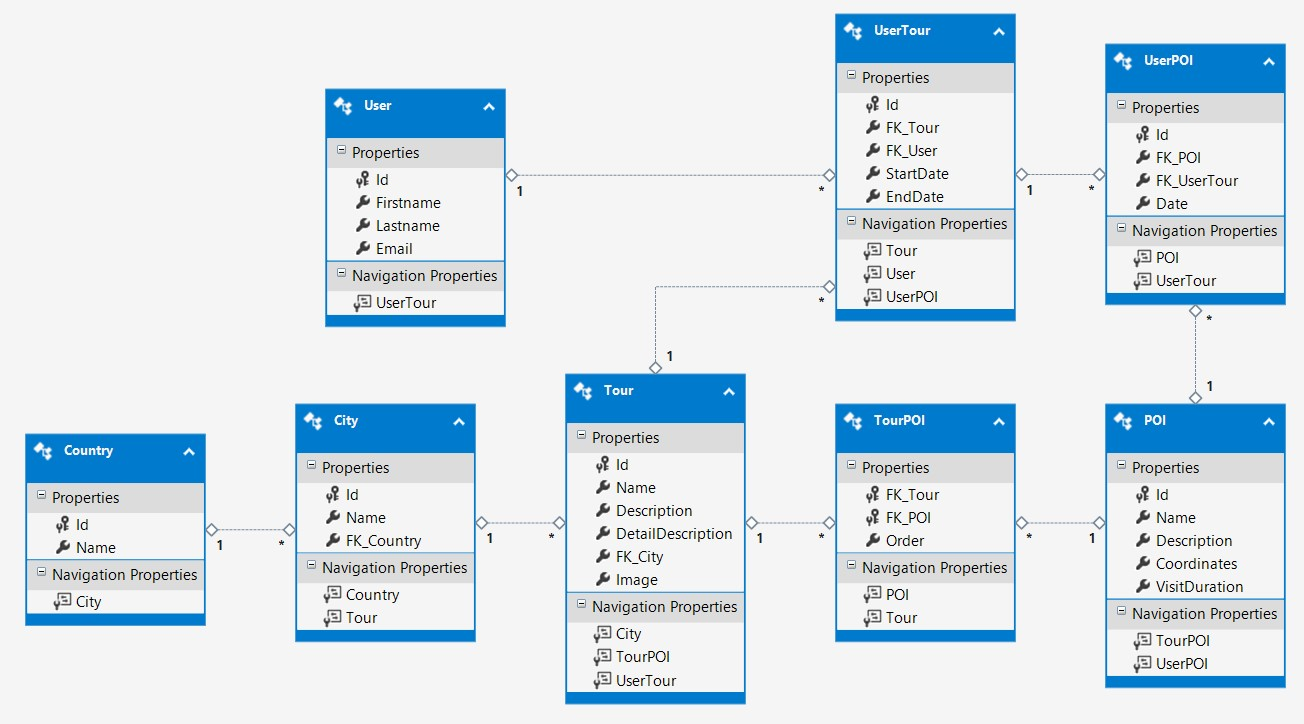
\includegraphics{erm_schlussbericht}
  \caption{Entity Relationship Diagram}
\end{figure}

\subsection{Frontend Design}\label{design-frontend}
Bei der Architektur und dem Design unterscheiden wir zwischen Backend
(Web Services) und dem Frontend (Android App). Beide Systeme werden parallel und
unabhängig mittels Swagger API Spezifikation entwickelt (siehe \fullref{service-api}).
Durch diesen Swagger Contract als klare Barriere lassen sich Entscheide betreffend
Architektur und Design separat treffen.
Zuerst behandeln wir das Frontend, danach das Backend.
\subsubsection{Design-Klassendiagramm}\label{design-klassendiagram}
\begin{figure}
  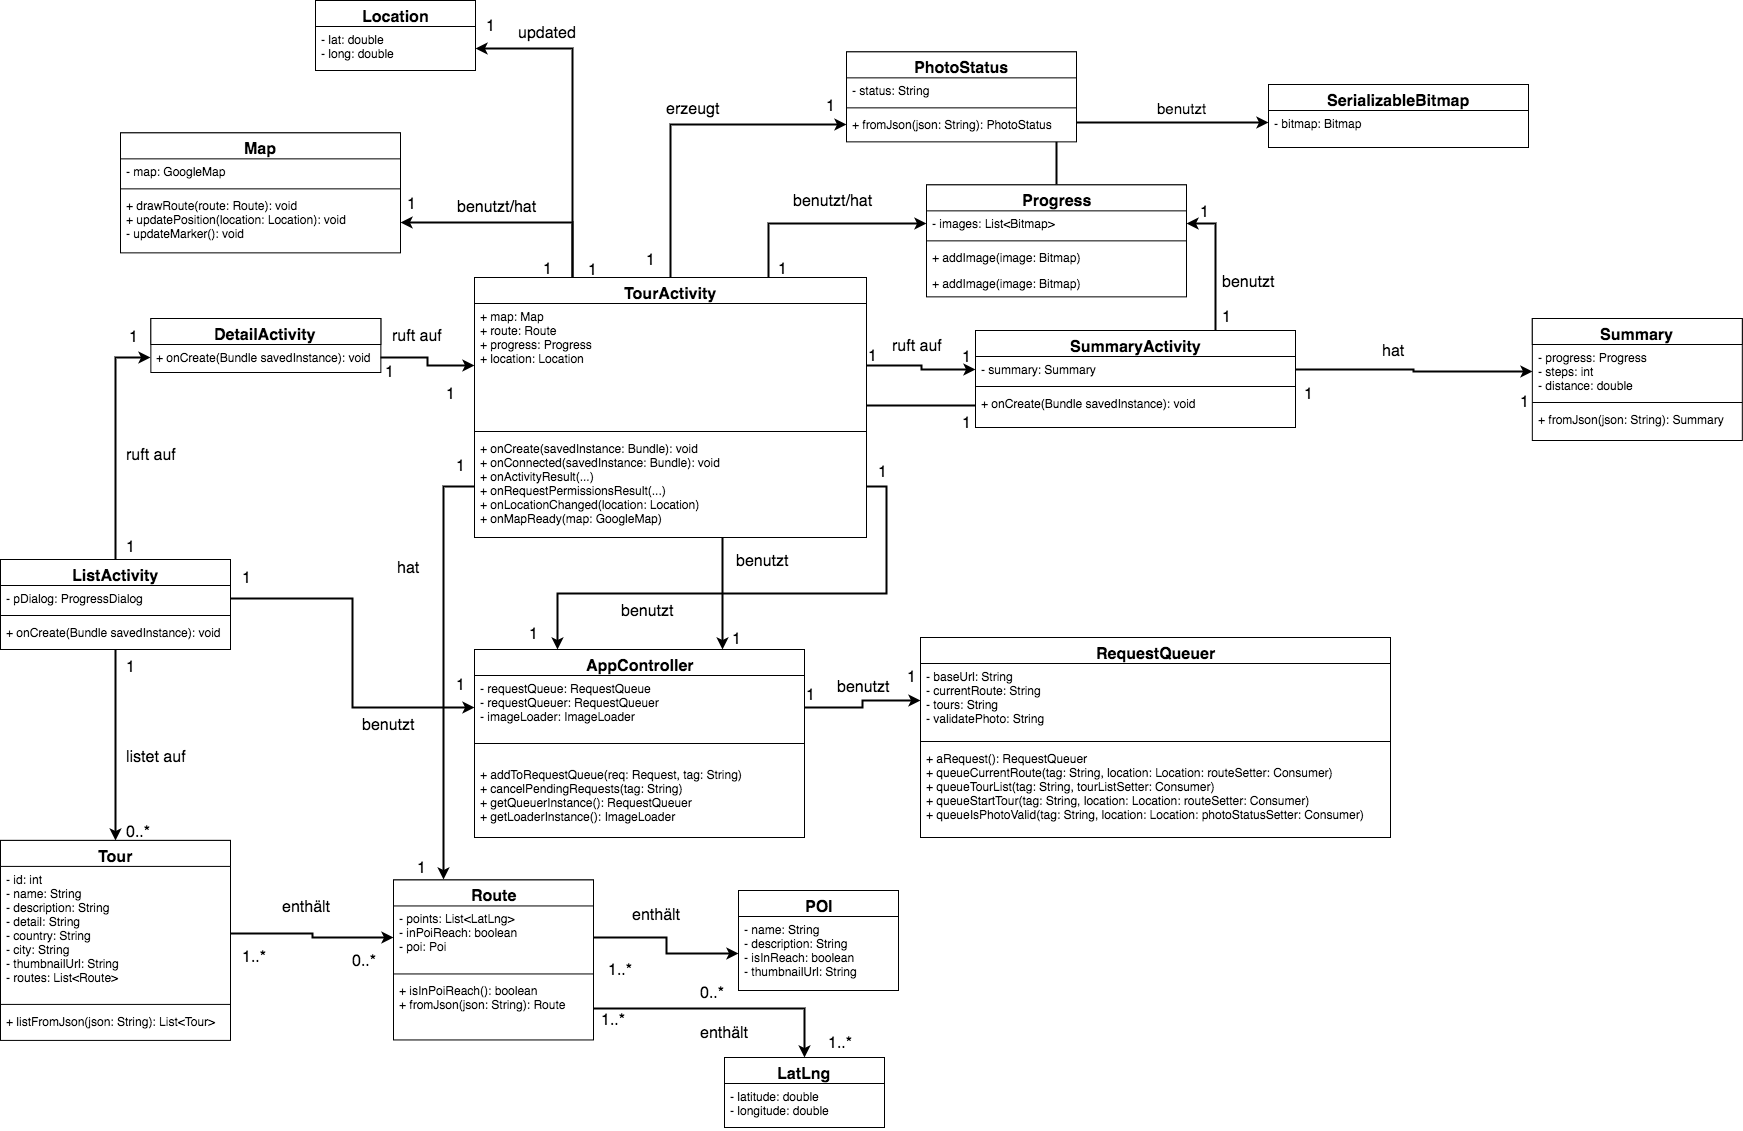
\includegraphics{classdiagram_frontend}
  \caption{Klassendiagramm der App}
\end{figure}

\newpage
\subsubsection{Klassenverantwortlichkeiten}\label{klassenverantwortlichkeiten}
In der folgenden Tabelle werden die Klassen mit ihren Hauptverantworlichkeiten
gelistet.

\begin{longtabu} to \textwidth { | l | X[l] |  }
\hline
\textbf{Klasse} & \textbf{Verwantwortlichkeit}\\\hline
\endhead
\textbf{AppController} & Der AppController liefert Instanzen von Singletons.\\\hline
\textbf{RequestQueuer} & Der RequestQueuer wird benutzt, um per HTTP mit dem
Server zu kommunizieren.\\\hline
\textbf{ListActivity} & Die ListActivity zeigt eine Liste von Touren an und
reagiert auf Klick-Events.\\\hline
\textbf{DetailActivity} & Die DetailActivity zeigt eine detaillierte Beschreibung
und ein Thumbnail einer Tour.\\\hline
\textbf{TourActivity} & Die TourActivity speichert die aktuelle Route, aktualisiert
die Position des Nutzers, aktualisiert die Karte und löst HTTP Requests aus.\\\hline
\textbf{SummeryActivity} & Die SummaryActivity erstellt eine \textbf{Summary}
und zeigt diese an.\\\hline
\textbf{Tour} & Die Tour kennt all ihre Routen und dient als Datenklasse. \\\hline
\textbf{Route} & Die Route kennt all ihre Koordinaten und dient als
Datenklasse. \\\hline
\textbf{POI} & Die POI ist eine reine Datenklasse und bildet ein POI ab.\\\hline
\textbf{LatLng} & LatLng ist ein Datentyp, welche eine Position auf dem
Erdball abbildet.\\\hline
\textbf{Map} & Die Map dient als Behählter der Google Map und wird benutzt, um
die Karte zu aktualisieren.\\\hline
\textbf{Location} & Location ist eine Repräsentation eines Ortes und kommt aus
Android SDK.\\\hline
\textbf{PhotoStatus} & PhotoStatus ist eine Datenklasse und repräsentiert das
Ergebnis einer Validierung eines Fotos durch das Backend.\\\hline
\textbf{Progress} & Progress dient als Behälter der während einer Tour geschossenen
Fotos.\\\hline
\textbf{Summary} & Summary wird am Ende einer Tour aus Progress generiert und
bietet dem Nutzer eine Zusammenfassung der Tour.\\\hline
\textbf{SerializableBitmap} & SerializableBitmap ist eine Wrapper-Klasse um ein Bitmap. Activities
kommunizieren untereinander mit Intents, welche einen serialisierbaren Anhang haben können.
Dadurch lassen sich Fotos zwischen Activities herumreichen.\\\hline

\end{longtabu}

\newpage
\subsubsubsection{Knowing and Doing}\label{knowinganddoing-frontend}
Im Folgenden betrachten wie die Knowing- und Doing-Verantwortlichkeiten der Klassen.
\begin{longtabu} to \textwidth { | l | X[2, l] | X[8, l] |  }
\hline
\textbf{Klasse} & \textbf{Knowing} & \textbf{Doing} \\\hline
\endhead
\textbf{AppController} & RequestQueuer & Stellt anderen Objekten den RequestQueuer
als Singleton zur Verfügung.\\\hline
\textbf{RequestQueuer} & keine Abhängigkeiten & Wird in den Activities für asynchrone
HTTP Kommunikation benutzt. Der RequestQueuer baut auch die URLs zusammen und bietet
eine API an, um mit Lambdas Callbacks zu setzen. Dieser ruft die mitgereichten
Consumer mit dem Server Response auf, ohne den Aufrufer zu kennen. Dadurch erreichen
wir lose Kopplung und hohe Wiederverwendbarkeit. \\\hline
\textbf{ListActivity} & AppController, Tour & Die ListActivity gibt über den AppController
einen Callback an den RequestQueuer. Dieser Callback füllt eine Liste von Touren,
welche dem User angezeigt wird. Ein Klick auf eine Tour ruft die DetailActivity auf.
\\\hline
\textbf{DetailActivity} & Tour & Die DetailActivity ist eine einfache Ansicht auf
ein Tour-Objekt und zeigt Details einer Tour an.\\\hline
\textbf{TourActivity} & Map, Route, Progress, Location, AppController & Die TourActivity bildet
unseren Haupt-Use-Case ab: Navigation per Karte durch eine Tour. Die TourActivity
registriert sich selber als Callback beim Google Maps Service und beim Google
Play Location Service. Weiterhin wird das Backend regelmässig nach der aktuellen
Route gefragt. Falls sich der User in der Nähe eines POIs befindet, wird die
Kamera App des Smartphones aktiviert.\\\hline
\textbf{SummeryActivity} & Summary, Progress, RequestQueuer & Die SummaryActivity
bekommt von der TourActivity ein Progress-Objekt. Nach einer Anfrage an das
Backend wird eine \textbf{Summary} Activity erstellt und angezeigt.\\\hline
\textbf{Tour} & Route & Die Tour kennt nur ihre Routen und dient als Datenklasse.
Sie kann sich selber aus JSON instanziieren.\\\hline
\textbf{Route} & LatLng & Die Route kennt all ihre Koordinaten und dient als
Datenklasse. Sie kann sich selber aus JSON instanziieren.\\\hline
\textbf{POI} & keine Abhängigkeiten & Die POI ist eine reine Datenklasse und bildet ein POI ab. Sie
kann sich selber aus JSON instanziieren.\\\hline
\textbf{LatLng} & keine Abhängigkeiten & LatLng ist ein Datentyp, welche eine Position auf dem
Erdball abbildet.\\\hline
\textbf{Map} & GoogleMap & Die Map dient als Behälter der Google Map und wird benutzt, um
die Karte zu aktualisieren. Sie kann den Positionsmarker und die Route zum nächsten
POI zeichnen.\\\hline
\textbf{Location} & keine Abhängigkeiten & kein Verhalten \\\hline
\textbf{PhotoStatus} & keine Abhängigkeiten & kein Verhalten \\\hline
\textbf{Progress} & keine Abhängigkeiten & kein Verhalten \\\hline
\textbf{Summary} & Progress & Summary kann sich selber aus \textbf{Progress}
generieren.\\\hline
\textbf{SerializableBitmap} & keine Abhängigkeitren & kann ein Bitmap serialisieren \\\hline

\end{longtabu}

Obwohl \textbf{Activities} andere \textbf{Activites} starten können, müssen sie
lediglich deren Klasse kennen. Durch das Messaging System von Android müssen die
Activities keine Instanzen von anderen Activities halten oder diese selber
erzeugen. Im Klassendiagramm (Abbildung 2) sind die Activities zwar miteinander
verbunden, aber durch das Message System (Intents) sind diese lose gekoppelt.


\subsubsection{Android App Architektur}\label{androidapparchitektur}

Die Architekur der App implementiert eine einfache Version von \textbf{The Clean Architecture} \cite{TCA}.
Im nachfolgenden Abschnitt werden einige wichtige Punkte von \textbf{The Clean Architecture}
erläutert, um die Implementation in TravelBuddy aufzuzeigen. Eine umfassende
Einleitung findet man bei Robert Martin (Uncle Bob) \cite{CC}.
\begin{figure}
  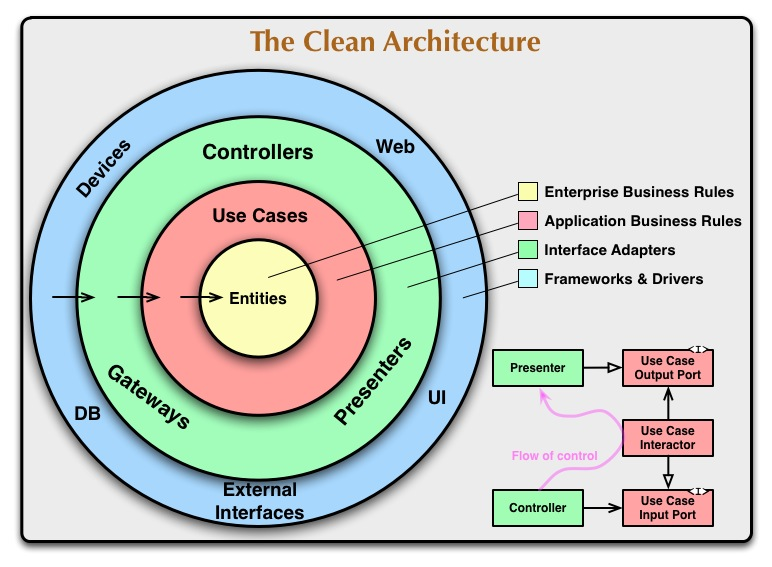
\includegraphics{cleanarchitecture}
  \caption{Schema von The Clean Architecture}
\end{figure}

\subsubsubsection{Abhängigkeiten - Dependency Rule}\label{dependencyrule}
Diese einfache Regel stellt lose Kopplung und gute Testbarkeit sicher.
Die \textbf{Dependency Rule} besagt, dass die Source Code Abhängigkeit nach innen zeigt.
Das heisst, dass eine bestimmte Schicht niemals die äussere Schicht kennt.
Man hat beispielsweise einen HTTP Client (Web) in der äussersten Schicht und
einen Parser (Gateway) in der direkt darunterliegenden Schicht. Nach der
\textbf{Dependency Rule} darf es keine Referenzen im Parser zum HTTP-Client geben.

\newpage
\subsubsubsection{Bedeutung der Schichten}\label{layers}
\begin{longtabu} to \textwidth { | l | X[l] |  }
\hline
\textbf{Bezeichnung der Schicht} & \textbf{Bedeutung und Beispiele}\\\hline
\endhead
\textbf{Frameworks and Drivers} & Die äusserste Schicht \textbf{Frameworks and Drivers}
ist für die Kommunikation mit der äusseren Welt zuständig. Dazu zählen zum
Beispiel Kommunikation mit dem User per UI, Persistierung von Daten in Datenbanken
oder Kommunikation mit externen Services per HTTP. Die äusserste Schicht beinhaltet
aber auch Frameworks.\\\hline
\textbf{Interface Adapters} & Die nachfolgende Schicht heisst \textbf{Interface Adapters}.
Diese Schicht hat zur Aufgabe, die Daten in eine für die Use-Cases- und Entities-Schicht
möglichst angenehme Form zu bringen.\\\hline
\textbf{Use Case} & Die zweitinnerste Schicht nennt man \textbf{Use Case} Layer.
Hier werden die applikationsspezifischen Businessregeln, also die Use Cases abgebildet.
Die eigentliche Businesslogik existiert also in dieser Schicht. Zu beachten ist aber,
dass es hier nur um Verhalten und nicht um Daten geht.\\\hline
\textbf{Entities} & Die eigentlichen Businessobjekte gehören in die innerste
Schicht, genannt \textbf{Entities}. Diese Schicht hat keine Abhängigkeiten zu
anderen Schichten und beinhaltet die generellen Regeln der Domäne. Bei Änderungen
in äusseren Schichten sind mit hoher Wahrscheinlichkeit keine Änderungen in dieser
Schicht notwendig. Zur Abgrenzung zur oberen Schicht \textbf{Use Case}: Die Schicht \textbf{Entities}
muss nicht angepasst werden, falls sich Use Cases ändern. Dies ist der Fall, da
sich die allgemeinen Domänenregeln in der Regel nicht ändern.\\\hline
\end{longtabu}

\subsubsubsection{The Clean Architecture bei TravelBuddy}
Die TravelBuddy App ist ein Spezialfall einer Android App. Da das Team das grösste
Risiko bei der Android-Entwicklung sah, wurde entschlossen, in der App selber so
wenig Businesslogik wie möglich auszuführen.
Dies hat natürlich einen Einfluss auf die Architektur, wie im folgenden Abschnitt aufgezeigt wird.

\begin{longtabu} to \textwidth { | l | X[l] |  }
\hline
\textbf{Schicht} &  \textbf{Zuständigkeiten und Beispiele} \\\hline
\endhead
\textbf{Frameworks and Drivers} & Kümmert sich um Lifecycle der App, die Berechtigungen
und um die Einbettung ins Android Betriebssystem, setzt HTTP Requests ab und reicht
HTTP Responses weiter, aktualisiert Standortdaten, bekommt Bilder von der
Smartphone-Kamera, erhält Karte von der Google Maps App\\\hline
\textbf{Interface Adapters} & Parst Antworten des Servers in String-Form und wandelt
diese Datenobjekte um, transformiert Kartendaten und Standortdaten in für die App
einfach zu handhabbare Form\\\hline
\textbf{Use Case} & Hier kommt der einfache Fall der Android App zugute: Die App
enthält sehr wenig Businesslogik. Die Use Cases sind im Backend implementiert.\\\hline
\textbf{Entities} & Enthält die Datenobjekte, welche die Domänenregeln abbilden:
Eine Tour besteht aus einer Liste von Routen, jede Route hat ein POI zum Ziel\\\hline
\end{longtabu}

\newpage
\subsubsubsection{Implikationen}\label{implications}
Die Anwendung der \textbf{Clean Architecture} bringt natürlich sowohl Vor- als
auch Nachteile. Die nachfolgende Liste zeigt Implikationen und Auswirkungen der
gewählten Architektur auf das Design und die Umsetzung der App.
\begin{enumerate}
  \item \textbf{Klare Abhängigkeiten:} Durch die klar definierten Abhängikeiten
    lassen sich Kosten und Aufwände von Änderungen/Erweiterungen besser abschätzen:
    Wollen wir beispielsweise die Technologie zur Kommunikation mit dem
    Backend von REST/HTTP auf WebSockets/PubSub ändern, wissen wir, dass sich
    die inneren beiden Schichten nicht ändern. Wir müssen lediglich die äussere
    Schicht anpassen, damit sie WebSockets handhabt. Der Parser, in der direkt
    darunterliegenden Schicht, erhält idealerweise den gleichen Response Body
    und muss nicht angepasst werden.
  \item \textbf{Gute Testbarkeit:} Die Businesslogik ist vollkommen unabhängig
    von verwendeteten Frameworks und der UI. Diese kann ohne eine laufende
    Android Instanz getestet werden. Das führt zu kürzeren Feedback Loops
    bei der Ausführung von Unit Tests und dadurch zur effizienteren Entwicklung
    (ein komplettes Re-deployment entfällt).
    Da in den beiden inneren Schichten keine Abhängigkeit zu externen Systemen
    besteht, lassen sich diese ohne grossen Aufwand (z.B. Testing-Setup) testen.
  \item \textbf{Keine Abhängikeit zum Betriebssytem:} Aus Punkt 1 und 2
    leitet sich dieser Punkt ab: Alle Abhängigkeiten befinden sich um
    äussersten Layer. Falls die App auch auf anderen Systemen lauffähig sein soll, dann muss im Idealfall nur eine Schicht angepasst werden. Durch Projekte wie RoboVM \cite{RV} und Intel Multi OS Engine \cite{MOE} können wir den bestehenden Java Code
    sogar auf iOS Geräten laufen lassen. Unsere App ist damit sogar nur lose
    zum Betriebssystem gekoppelt.
  \item \textbf{Overhead:} Da die App in der ersten Version praktisch keine
    Businesslogik enthalten wird, entfällt die \textbf{Use Case} Schicht.
    Dadurch bleiben eigentlich die anderen drei Layer, die mit der ersten
    Version ebenfalls noch überschaubar ausfallen. Man könnte argumentieren,
    dass diese Architektur etwas zu hoch gegriffen ist für die Anforderungen
    des Prototypen. Im Gegensatz zu Design lässt sich Architektur nicht oder
    sehr schwer inkrementell entwickeln. Wir denken, dass der Aufwand für Änderungen
    der Architektur im späteren Verlauf (etwa durch neue Anforderungen) den
    initialen Mehraufwand rechtfertigt.
\end{enumerate}

Durch die gewählte Architektur erreichen wir gute Testbarkeit mit klaren
Abhängigkeiten. Der Mehraufwand wird dadurch gerechtfertigt, dass Änderungen
von Technologien nur kleine, kalkulierbare Anpassungen zur Folge haben.

\subsubsubsection{Tatsächliche Umsetzung}\label{implementation_frontend}
Die tatsächliche Implementation weicht leicht von der geplanten Architektur ab. Das Team hat den
Aufwand zur vollständigen Entkopplung der äussersten Schicht \textbf{Frameworks and Drivers} abgeschätzt
und schliesst, dass der Mehrwert in diesem Fall den Schritt nicht rechtfertigt.

Im die \textbf{Frameworks and Drivers} vom Rest der App zu entkoppelt, müssten viele Helper-, Wrapper- und
Facaden-Klassen eingeführt werden. Da die Aufrufe von externen Libraries wie dem HTTP Client Volley
oder der JSON-Parsing Library GSON nur punktuell stattfinden, nehmen wir die Verletzung der \textbf{Dependency Rule}
bewusst in Kauf.
Die vollständige Entkopplung der \textbf{Frameworks and Drivers} kann, wenn auch mit mehr Aufwand,
zu einem späteren Zeitpunkt durchgeführt werden. Dieser Punkt gehört definitiv zu den Erweiterungsmöglichkeiten
und ist ab einer gewissen Grösse des Projekts obligatorisch

Die Wahl von guten Abstraktionen und Einhaltung der \textbf{Dependency Rule} ist uns hingegen bei den beiden
inneren Schichten gelungen. Nur durch Betrachten der \textbf{Entitites} werden die Domänenregeln sofort klar,
die Klassen selber haben alle geringe bis keine äusseren Abhängikeiten.
Die \textbf{Use Case} Schicht ist teils in den Activities verwoben. Dies akzeptieren wir bewusst,
da die Businesslogik grösstenteils auf dem Server stattfindet und die Activities auf Input reagieren.
Ausserdem bestehen die Activities fast ausschliesslich aus einer Auflistung von registrierten Callbacks,
was der Lesbarkeit des Codes nicht schadet.

\newpage
\subsubsubsection{Activities}\label{activities}
Die App selber besteht aus drei Haupt-Activities. \textbf{Activities} ist ein
Konzept von Android, sie bilden eine User-Ansicht ab und bilden des Skelett
der App. Abbildung 4 veranschaulicht alle möglichen Zustände und deren
Änderungen.
\begin{figure}
  \centering
  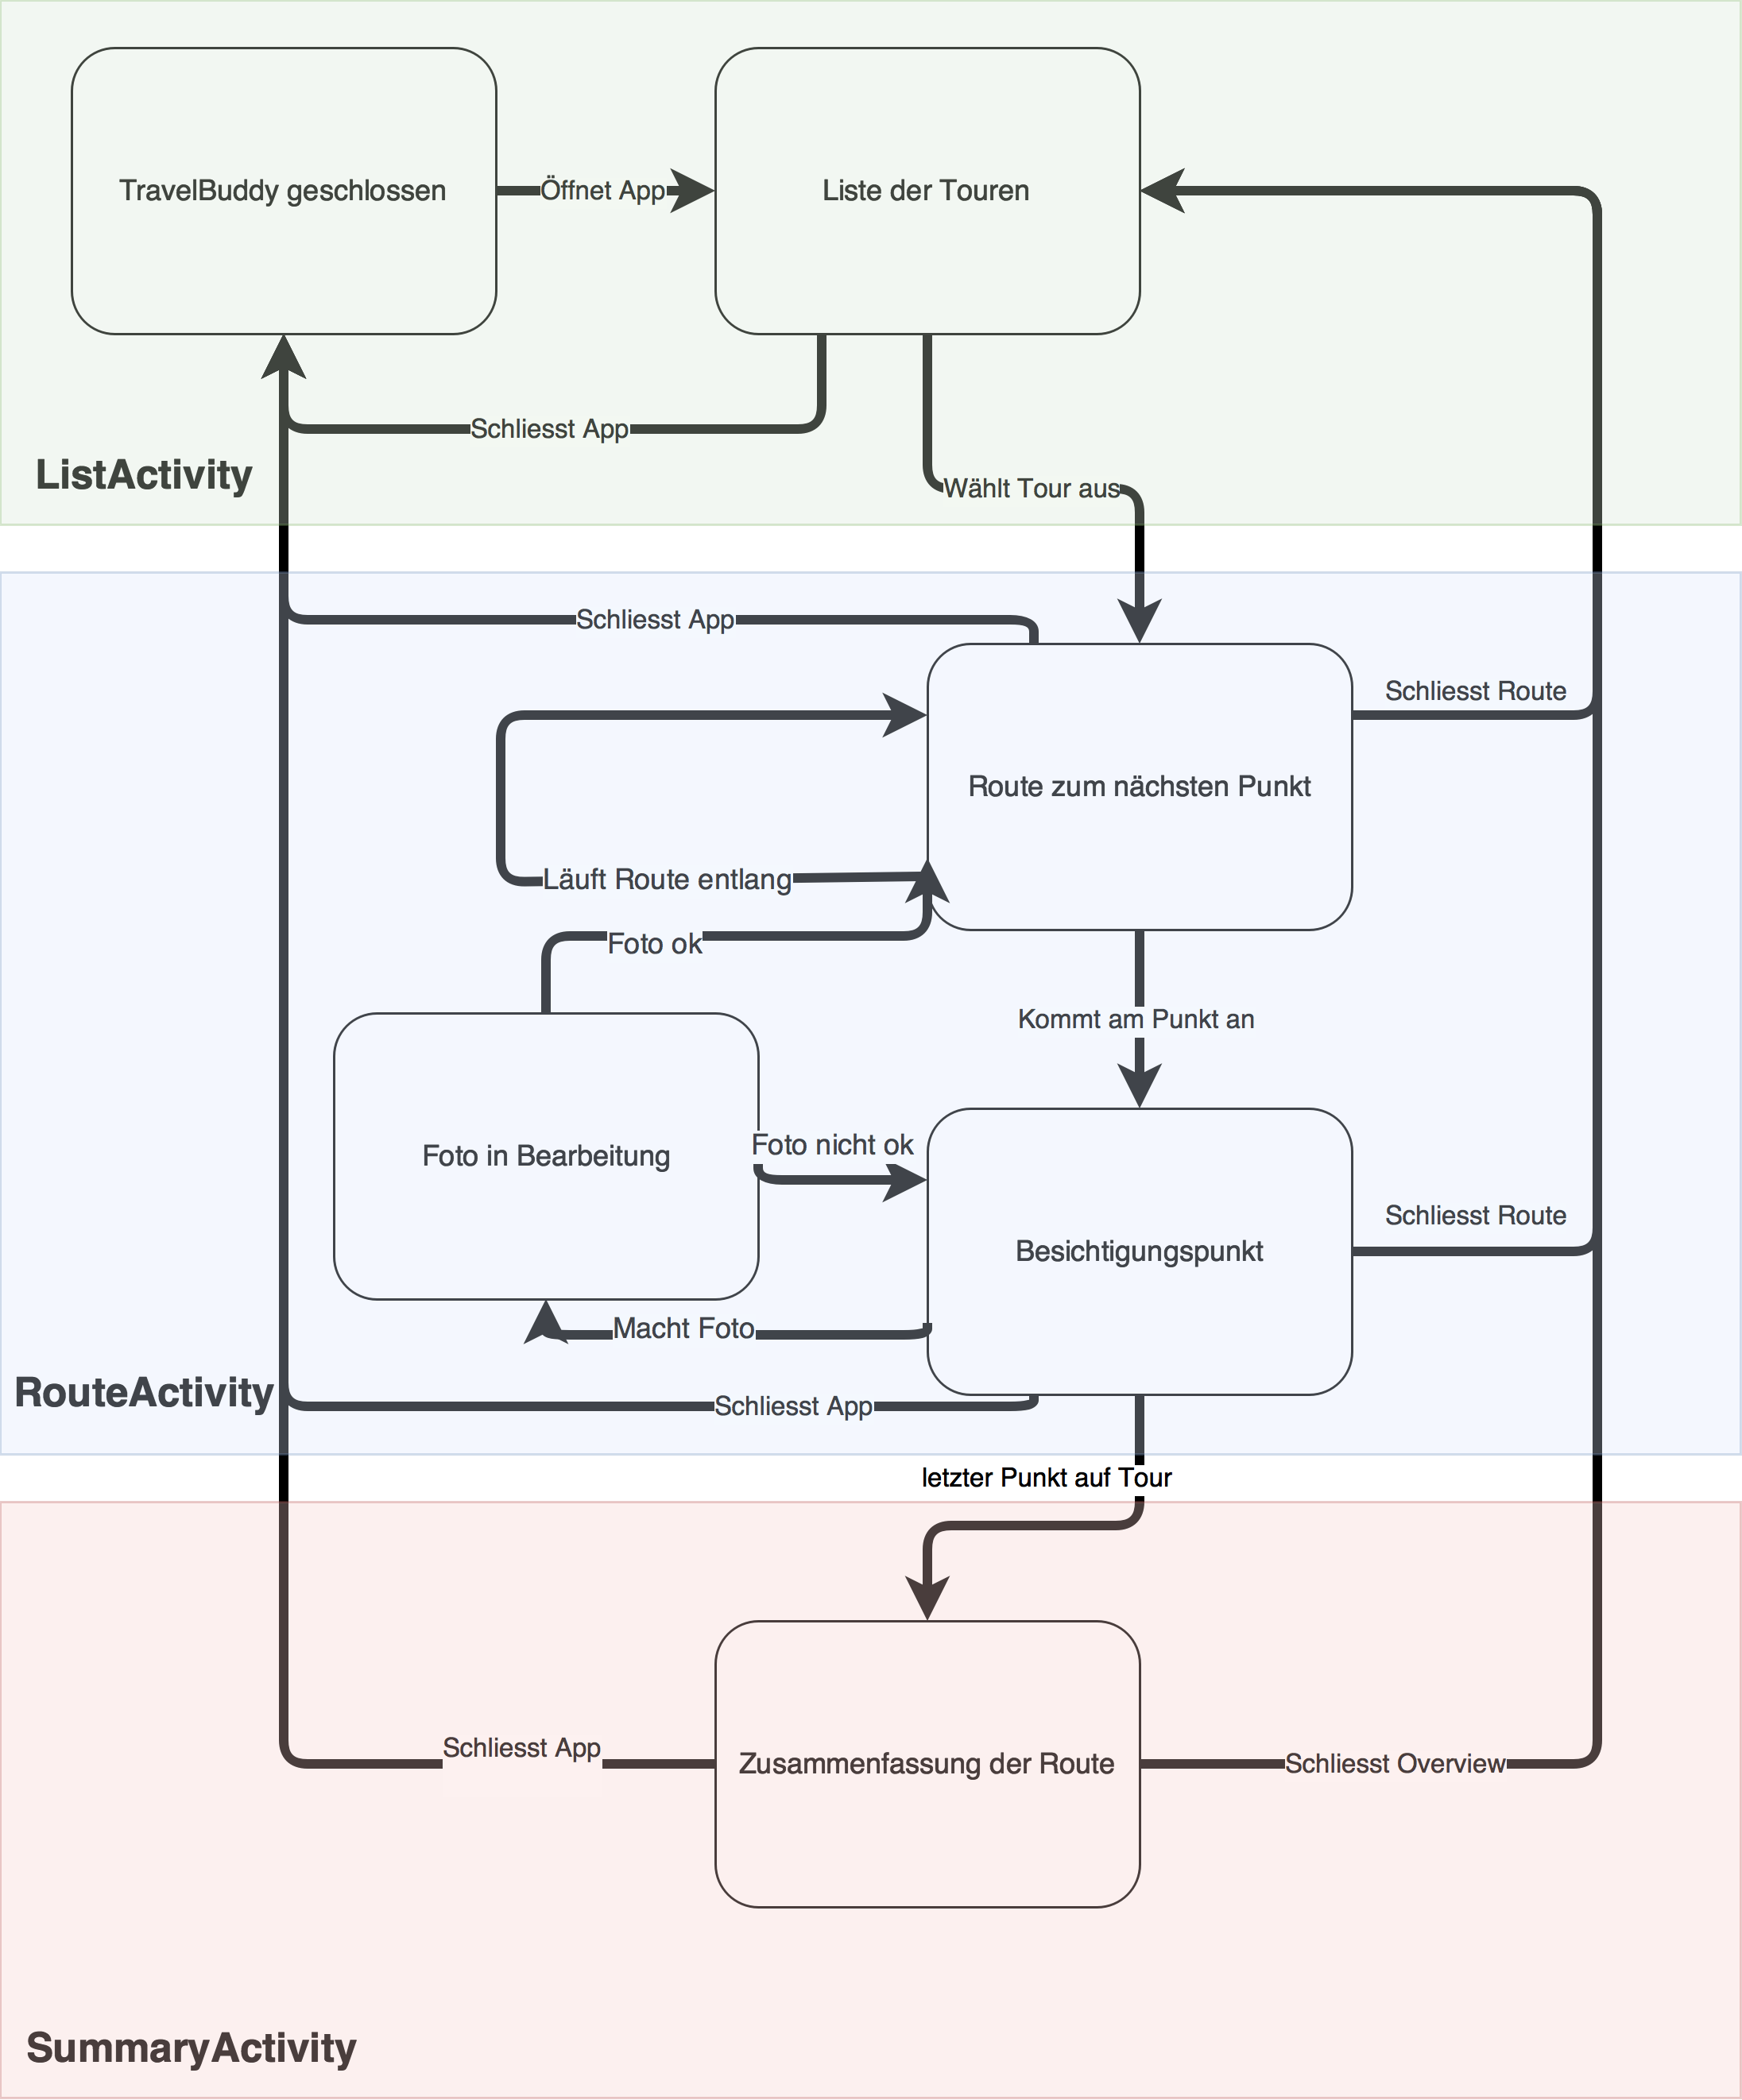
\includegraphics[height=19cm]{state-diagram}
  \caption{Zustandsänderungsdiagramm}
\end{figure}


\section{Implementation}
\subsection{Testbericht Backend}\label{backendTestbericht}
Das Backend wurde isoliert von der Android-App manuell getestet. Zu diesem Zweck wurde Swagger verwendet. Swagger stellt eine Bedienoberfläche bereit, mit welcher man alle Funktionen der Travelbuddy API testen kann. Um das Backend testen zu können, mussten vorher Beispiel-Daten erfasst werden. Diese wurden ebenfalls für das Testen der Android-App und Demozwecke verwendet. Da wir keine Applikation zum Erfassen von Touren entwickeln, mussten die Daten direkt über die SQL-Datenbank erfasst werden. Beim Testen der API wurde jede einzelne Funktion aufgerufen und überprüft, ob das korrekte Resultat vom Backend zurückgegeben wurde. System- und Integrationstests wurden dadurch im Selben durchgeführt. Denn diese Tests gaben Aufschluss darauf, ob die Kommunikation mit der Google-Maps API und der Datenbank richtig funktionierten. Einfachheitshalber haben wir auf ein Ticketing-System verzichtet. In Zukunft müssten aber die Issues in einem System verwaltet werden. In diesem Stadium des Projekts war dies allerdings nicht nötig. Fehler die von den Android-App-Entwickler entdeckt wurden, haben diese direkt an die Backend-Entwickler via Slack kommuniziert. Diese Kommunikation funktionierte gut und dadurch konnte sehr rasch auch auf Änderungswünsche bezüglich der API eingegangen werden.

Um bei Änderungen oder Erweiterungen am Backend sicher zu sein, dass die bestehende Funktionalität nicht negativ beeinflusst wurde, haben wir für die wichtigsten Funktionen Unit-Tests geschrieben. Nachfolgend einer Zusammenfassung der umgesetzten Unit-Tests und deren Testresultat. Zum Zeitpunkt des Code-Freeze am 15. Mai 2017 laufen alle Unit-Tests erfolgreich durch.

\begin{figure}
  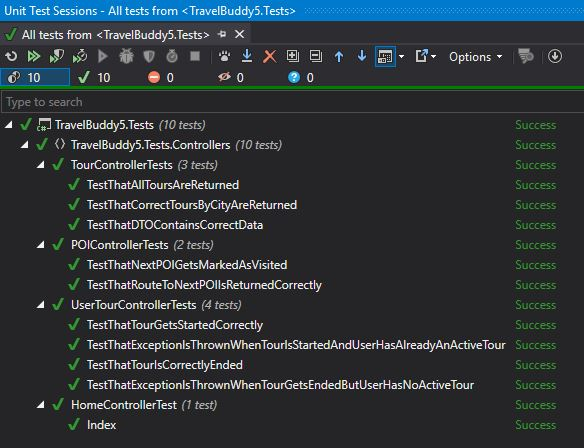
\includegraphics{backend_unit_test_summary}
  \caption{Unit-Test-Bericht Backend }
\end{figure}

\subsection{Testbericht Frontend}\label{testbericht_frontend}
Nachfolgend wird auf das Testing der Android App eingegangen.

\subsubsection{Automatisiertes Testen}\label{automatisiertes_test_frontend}
Es war bereits zu Beginn des Projekts klar, dass es eine Aufteilung in Frontend und Backend
gibt. Da in unserem Team das Android Know-How begrenzt ist, haben wir uns dazu entschieden,
möglichst viel Logik auf dem Backend auszuführen und die Android App so klein wie möglich zu halten.

Da die App ohne Server nicht funktional ist, mussten wir Teile der App schon zu Beginn an
Test-Driven zu entwickeln. Mithilfe des Swagger Contracts haben sowohl das Frontend- als auch das
Backend-Team gegen die selbe API entwickelt. Dadurch konnte das Frontend-Team Antworten des Servers
als Mock in Unit-Tests einbauen und so schon früh Funktionalitäten wie Parsing und das Bauen der URL
testen. Die App selber enthält keine Business-Logik, die getestet werden kann. Dadurch beschränkt sich
auch das automatische Testen auf das Parsen von Server-Antworten und das Aufrufen von URLs.

Für CI (\textbf{Continous Integration}) verwendet das Frontend-Teams travis-ci.org 
(\url{https://travis-ci.org/PsitTeam3/TravelBuddyAndroidApp}). Dieser führt alle Tests
aus und baut das komplette Projekt, wenn ein Entwickler committed. Durch die Kombination von \textbf{Linting}
und den \textbf{Unit-Tests} konnten wir schon frühr Probleme erkennen und beheben.

Auf Integrations-Tests wurde hier verzichtet, da die Integration von Umsystemen von Android erledigt
wird. Sowohl der HTTP-Client als auch Google Maps Services funktionieren ohne Konfiguration. Auch hätte
dies einen nicht gerechtfertigten Mehraufwand bei der Infrastruktur (CI) bedeutet, da die Ausfühung
solcher Tests eine laufene Android-Instanz benötigt. Wäre die Integration der Umsysteme kein solches
"Out-of-the-box"-Erlebnis, dann hätten wir Aufwand in Integrations-Tests gesteckt.

\subsubsection{Manuelles Testen}\label{manuelles_testen_frontend}
Natürlich ist bei einer mobilen Applikation des manuelle Testen sehr wichtig, denn nur damit lassen
sich Probleme beim User-Erlebnis (User Experience/UX) finden. Gegen Ende der Construction Phase
hatten sowohl Backend als auch Frontend beide genug Funktionalität, um die ersten Use Cases zu testen.

Die Use Cases dienten dabei als \textbf{Soll}, das es zu erreichen gilt. Zusätzlich wurde die Anforderung
gestellt, dass der Benutzer unerwartete Handlungen vornimmt, wie z.B. Schliessen/Minimieren der App oder
unerwartete Rückwärts-Navigation. Beim manuellen Testen wurden solche Szenarion provoziert, unter anderem
durch:

\begin{enumerate}
  \item Langes Verweilen in Screens (Timeout)
  \item Sehr schnelles/ungeduldiges Bedienen der App
  \item Minimieren/Schliessen der App
\end{enumerate}

Es wurde eine Test-Tour angelegt, mit zwei POIs, die etwa 400m voneinander entfernt sind. Dann wurde
eine Route, welche beide POIs enthält zur Simulation der GPS Koordinaten im Android Emulator verwendet.
Dabei sendet der Emulator der App alle zwei Sekunden den nächsten Wegpunkt als Koordinate und emuliert
so einen User, der durch die Stadt spaziert. So wurde Funktionen wie das Fotografieren von POIs, das
Erledigen von Routen und die Berechnung der aktuell schnellsten Route als Fussgänger getestet.

Da die App nur im Emulator getestet wurde, kann man argumentieren, dass diese Tests sehr synthetisch
sind und nicht den Bedingungen der "echten Welt" entsprechen. Dies wurde bewusst so durchgeführt, da
der Prototyp die Sinnvolligkeit der Domänenregeln und die Umsetzbarkeit mit den gewählten Technologien
beweisen soll.
Ausserdem übernimmt Android auf Betriebssystem-Ebene sehr viel, das man sonst auf Applikations-Ebene
machen müsste. So stellt Android beispielsweise eine Facade zur Verfügung, um den letzten bekannten
Standort abzufragen. Dabei werden intern mehrere Datenquellen angezapft, bewertet und prioritisiert.
Dies käme nur in einem Test auf einem echten Gerät z.B. in der Stadt zum Zug. Wir glauben, dass dadurch
Tests mit dem Emulator ausreichen und etwaige Anpassungen nach einem Test unter echten Bedingungen
miniaml sind.

\subsubsection{Resultate}\label{test_resulate}
Alle geplanten \textbf{Uses-Cases} sind implementiert und sind in der ersten Version komplett. Sogar
ungeplante alternative Szenarien innerhalb der Use-Cases funktionieren. Durch die korrekte Implementation
der Lifecycle-Hooks der Activities kümmert sich Android um das Minimieren und das "Zurücknavigieren".

Das \textbf{UI} entspricht in etwa den zu Beginn erstellen Mockups und den Erwartungen. Das Theme passt
farblich zu unserem Corporate-Branding und die Animationen/Menüs sind zeitgemäss.

Die \textbf{Stabilität} stufen wir als genügen ein. Da die App selber wenig Logik hat, ist die Lauffähigkeit
stark vom Server abhängig. Bei serverseitigen Ausfällen bleibt die App zwar meist stabil, der User
bekommt aber keine Meldung. Dieser Punkt hat starken Einfluss auf das User-Erlebnis (UX) und müsste
vor einem öffentlichen Release unbedingt nachgebessert werden.


\section{Resultat}\label{resultat}

\subsection{Erreichte Ziele}\label{erreichteZiele}

Die Ziele welche wir uns für die Umsetzung des Projekts im Rahmen des PSIT3 Moduls gesetzt haben, wurden alle erreicht:
\begin{itemize}
  \item Eine Liste mit allen verfügbaren Touren kann angezeigt werden.
  \item Eine Tour kann von der Liste gewählt und gestartet werden.
  \item Die App sendet an das Backend die Koordinaten der Reisenden. Das Backend ist mit dieser Information in der Lage, eine Anfrage an die Google-Maps API zu stellen und die Route zu einem Besichtigungspunkt der Tour zurückzugeben.
  \item Die Kartenfunktionalität wurde erfolgreich implementiert. Die Karte zeigt die Route zum nächsten Ziel. Dabei wird die Route für die Fortbewegung zu Fuss angezeigt. Dem Kunden wird keine andere Möglichkeit angezeigt, wie er an das Ziel gelangen kann. Ursprünglich war hier die Idee, dass der Touristin verschiedene Optionen angezeigt werden, unter anderem die Integration von Uber.
  \item Während dem sich die Reisende fortbewegt, wird die Route periodisch angepasst.
  \item Die App erkennt, wenn der Reisende sich in der Nähe des Ziels befindet und es werden sofort die Informationen zu dem Besichtigungspunkt eingeblendet.
  \item An einem Besichtigungspunkt angekommen, wird der Tourist ebenfalls aufgefordert, ein Foto eines bestimmten Objektes zu schiessen. All diese verschiedenen Fotos werden lokal gespeichert und später für die Zusammenfassung der Tour verwendet.
  \item Am Ende der Tour wird dem Touristen eine Zusammenfassung seiner Tour angezeigt, welche unter anderem die persönlichen Fotos der Tour enthält.
\end{itemize}

Die Travelbuddy API, das Backend-System, erfüllt alle funktionalen Anforderungen, welche durch den Umfang der Android-App gegeben sind. Das beudetet, dass die Android-App bereits alle benötigten Daten von der API beziehen kann. Das Backend ist auch bereits an einen SQL-Server angebunden, um die Daten zu persistieren.


\subsection{Offene Punkte}\label{offenePunkte}
Einige Punkte der Projektidee standen nicht im Fokus und sind darum noch offen:

\begin{itemize}
  \item Die Fotos welche die Anwenderin während der Tour macht, werden nur lokal auf dem Gerät gespeichert. Die Fotos sollten aber an das Backend gesendet werden, damit die Fotos persistiert werden, aber auch von einem anderen Gerät her abgefragt werden könnten.
  \item Die Benutzerauthentifizierung fehlt noch komplett. Die App funktioniert aktuell nur für einen Benutzer. Das Backend ist jedoch schon für die Verwendung mehrerer Anwender vorbereitet. Über die API ist es möglich, Touren für verschiedene Benutzerinnen zu starten. Dazu werden für die verschiedenen Aufrufe jeweils eine Benutzer-ID als Parameter mitgegeben. Es fehlt jedoch auch noch die Authentifizierung auf Backend-Seite, da noch keine Passwörter vorgesehen sind, bzw. kein Passwort-Hash zusammen mit der Benutzer-ID mitgegeben werden kann.
  \item Touren können nicht gefiltert werden, es wird lediglich eine Liste mit allen verfügbaren Touren angezeigt.
  \item Die personalisierte Zusammenfassung der Tour bei Tourbeendung kann nicht auf einem Social-Media Account geteilt werden.
  \item Eine gestartete Tour kann nicht unterbrochen oder abgebrochen werden. Wenn der Tourist die App schliest, kann die Tour nicht fortgesetzt werden.
\end{itemize}


\subsection{Weiterentwicklungsmöglichkeiten}\label{weiterentwicklungsmöglichkeiten}
Nachfolgend einige Ideen, wie das Travelbuddy-Projekt fortgesetzt werden könnte:
\begin{itemize}
  \item Zur Berechnung der Route fragt die Android-App das Backend an, die Route vom aktuellen Standort der Touristin zum nächsten Punkt zurückzugeben. Das Backend wiederum macht daraufhin eine Anfrage an Google-Maps. Da dies periodisch in kurzen Zeitintervallen geschieht, ist dies nicht besondern performant. Besser wäre es, wenn der Client die Route gleich selbst bei Google-Maps abfragt.
  \item Die Integration von Uber war in der Projektidee enthalten, wurde aber in der Anforderungsanalyse verworfen. Dies wäre aber ein für die Touristen hilfreiches Feature.
  \item Grosses Potential sehen wir im Bezug auf Augmented Reality. Es wäre genial, wenn man während einer Tour auf dem Gerät Informationen über interessante Objekte angezeigt bekäme, welche gerade im Sichtfeld des Anwenders sind. Also wenn die Anwenderin z.B. eine Tour durch das Niederdorf in Zürich macht und in der Nähe des Grossmünsters ist, würde auf dem Gerät das Grossmünster abgebildet werden und gleich dazu Informationen über die Kirche und allenfalls auch gleiches für den Brunnen daneben und das Café gegenüber. Man könnte das Konzept auch sehr gut für Museen verwenden, wo man unter Verwendung einer Holo-Lens digital geführte Touren durch das Museum oder eine Ausstellung anbieten könnte. Mit einer Holo-Lens könnte eine Applikation geschrieben werden, welche die verschiedenen Gegenstände erkennen und Informationen in beliebiger Form in den Raum projezieren kann. Um diese Idee umzusetzen würde am besten ein platformunabhängiges Framework entwickelt werden. Darauf aufbauend könnten verschiedene Client-Applikationen für unterschiedliche Geräte und auch unterschiedliche Zwecke (Museums-Tour, Städte-Tour, Gebäude-Tour für grosse Neubauten und vieles mehr) entwickelt werden.
  \item Eine Web-Applikation wäre hilfreich für die Tourvorbereitung, sowie für das Ansehen der Tour-Zusammenfassungen. Es könnte also zusätzlich eine Web-Oberfläche umgesetzt werden, mit welcher der Tourist an seinem Computer Zuhause alle verfügbaren Touren für seine Feriendestination durchgehen und diejenigen speichern könnte, welche er schlussendlich durchführen möchte. Diese Arbeit ist produktiver an einem Laptop oder Computer als auf einem Smartphone oder Tablet. Zudem könnte die Oberfläche ebenfalls so gestalltet werden, dass die Touristin nach Beendigung einer Tour dort ihre persönliche Zusammenfassung inlusive ihrer Fotos anschauen und auch auf einem Social-Media Profil teilen könnte.
  \item Touren können momentan nur direkt via SQL erfasst werden. Das ist unpraktikabel. Sämtliche Daten müssten mit Hilfe einer Web-Oberfläche erfasst werden können. Dazu müsste eine eigene Web-Applikation entwickelt werden, die dann auch von Reisebüros verwendet würde.
\end{itemize}


\addcontentsline{toc}{section}{Literatur}
\begin{thebibliography}{9}
  \bibitem{TCA} URL: https://8thlight.com/blog/uncle-bob/2012/08/13/the-clean-architecture.html [Stand: 20.4.2017]
  \bibitem{CC} URL: http://blog.cleancoder.com/ [Stand: 20.4.2017]
  \bibitem{RV} URL: http://robovm.mobidevelop.com/ [Stand: 20.4.2017]
  \bibitem{MOE} URL: https://software.intel.com/en-us/multi-os-engine [Stand: 17.4.2017]

  \bibitem{TomasCookApp}
    Thomas Cook Travelguide in Goggle Play [Online].
    URL: https://play.google.com/store/apps/details?id=com.tc.android.travelguide\&hl=de [Stand: 4.3.2017].

  \bibitem{UberApi}
    Uber Integration für Apps [Online].
    URL: https://developer.uber.com/products/ride-requests [Stand: 4.3.2017].
\end{thebibliography}

\section*{Abbildungsverzeichnis}\label{abbildungsverzeichnis}
\addcontentsline{toc}{section}{Abbildungsverzeichnis}
\begingroup
\renewcommand{\section}[2]{}%
\hypersetup{linkcolor=black}
\listoffigures
\endgroup

\end{document}
